\documentclass[12pt]{article}

\usepackage{amsmath} 
\usepackage{verbatim}
\usepackage{amsfonts}
\usepackage{indentfirst}
\usepackage[shortlabels]{enumitem}
\usepackage{graphicx}
\usepackage{epstopdf}
\usepackage{float}
\usepackage[T1]{fontenc}
\usepackage{lmodern}
\usepackage{subcaption}

\addtolength{\textwidth}{2cm}
\addtolength{\hoffset}{-1cm}
\addtolength{\textheight}{2cm}
\addtolength{\voffset}{-1cm}

\pagestyle{myheadings}
\markright{\hfill TIES Second Year Paper \hfill}
\title{Does Access to Healthcare Matter for Entrepreneurship?}
\author{Ankur Chavda}

\begin{document}
\maketitle

\begin{abstract}
We study the effect of improved access to health insurance on entrepreneurial rates across industries. We use the 2006 reform of the Massachusetts health care market as our shock. In contrast to previous research, we use our shock to test which kinds of startups were more likely to be created in addition to whether individuals became more likely to become entrepreneurs.  We develop a theoretical model uses institutional heterogeneity to make predictions on how the reform should affect the distribution of entrepreneurs across industries. We see evidence that although non-profit entrepreneurship was significantly affected, overall entrepreneurship is constrained by factors other than access to health care. 
\end{abstract}


\section{Introduction}
Traditionally health insurance in the US has been tied to employment through group plans. In 2013, only 17\% of Americans with private insurance\footnote{Non-private insurance is composed of Medicare, Medicaid and military health care} obtained it through the individual market \cite{census}. The differences between group and individual insurance are material for entrepreneurs leaving employment to start their own firms. Those that need coverage on the individual market face higher premiums or even the inability to purchase health insurance \cite{kaiser}. Uncertainty is also greater on the individual market; it is more likely for a person with an individual plan to lose insurance than someone under a group plan \cite{pauly}. 

Concerns over access to health care may be dissuading potential entrepreneurs from creating new firms. As one entrepreneur writes:
\begin{quote}
Obamacare affected me in another critical way as well. Its assurance of a stable insurance market that does not screen out someone with a pre-existing condition made me far more comfortable starting my own business. It gave me a baseline of security that simply didn't exist before. It helped make entrepreneurialism possible. \cite{sullivan}
\end{quote}

The literature on this topic focuses on answering how potential entrepreneurs are affected by access to health insurance. Early work by Holtz-Eakin, Penrod and Rosen \cite{holtz_health}  estimated the propensity to become self-employed as a function of access to health insurance. More recent work refined these types of estimates for specific sub-populations; Fairlie, Kapur and Gates \cite{fairlie_health} is an example that uses different datasets to generate estimates by sex and for workers nearing retirement. We are deepening our understanding of how access health insurance impacts various types of entrepreneurs. 

We are not aware of research asking the complementary question of what potential \emph{enterprises} are affected by access to health insurance. To illustrate, consider the response of one high-tech entrepreneur in Cambridge, MA when probed about the entrepreneurial impact of the 2006 health insurance reform in Massachusetts:
\begin{quote}
[The] top barrier[s] to people starting companies are [a] lack of drive and lack of capital ... it takes a lot of drive to start companies, and lack of healthcare is too small a barrier compared to others. For some freelancer[s] I think healthcare does help.
\end{quote}
The above quote suggests we will see an effect in single person consulting companies but not in high growth startups. More generally, the impact of health care reform may vary by type of firm and not just by type of entrepreneur. 

In this paper we contribute to the literature in two ways. First, we show by example that using heterogeneity in firm characteristics can increase our ability to produce significant results in otherwise challenging quasi-experimental settings. Second, our example results are interesting in their own right; they broaden our understanding of what influences the rate of entrepreneurship. 

Specifically, we take advantage of variation in the two requirements for entrepreneurship called out in the above quote: drive and capital. We use a firm's tax status to generate insights about drive; higher tax rates should reduce overall incentives to start firms and therefore mitigate entrepreneurial drive. We also develop a theoretical model that shows how start-up capital requirements can inform us about whether entrepreneurs are in fact constrained by access to health care. Our results suggest that while health care reform may provide marginal benefits to general entrepreneurship and stronger benefits to non-profit entrepreneurship, in general health care is not a effective policy lever to influence the level of entrepreneurship in an economy.

The rest of the article proceeds as follows. Section \ref{sec:review} reviews our current knowledge on the importance of both access to health care and entrepreneurship. Section \ref{sec:reform} describes the Massachusetts health reform we use as a policy shock. Section \ref{sec:model} outlines a model that considers how the reform should heterogeneously affect entrepreneurship by industry. Section \ref{sec:data} describes the data sources we use in our analysis. Section \ref{sec:regression} explains our empirical approach. Section \ref{sec:results} presents the effects of the reform on entrepreneurship and Section \ref{sec:conclude} concludes. 

\section{Literature Review}
\label{sec:review}

The importance of health insurance to economic rather than pure health outcomes was first explored by labor market researchers. Their motivation was to understand what is commonly referred to as ``job lock'': inefficiencies in matching workers to jobs due to non-portable benefits. Early findings suggested job lock due to health insurance was significant. Madrian \cite{madrian} for example estimated that health insurance job lock reduced voluntary turnover by 25\%. More recent work has continued to find significant results with real implications for policy makers. Garthwaite et al. \cite{garthwaite} argue that providing free health insurance to poor, childless Americans is a bad idea; they estimate it would reduce the US labor force by over half a million workers. 

Entrepreneurship researchers shifted the scope of this investigation by in effect asking: we know healthcare matters for labor markets, but what about new firm creation? This is arguably an equally important economic outcome to consider, for example Haltiwanger et al. \cite{haltiwanger} has recently pointed out that startups account for a disproportionate amount of new job creation in the US. However in contrast to the job lock literature, the study of entrepreneur lock has produced less consistent results. 

Holtz-Eakin et al. \cite{holtz_health} were the first to ask this question and found no strong relationship using both variance in spousal insurance coverage and the COBRA regulation\footnote{Consolidated Omnibus Budget Reconciliation Act (COBRA) of 1985} requiring the ability to continue coverage after employment ends. More recent work by Bailey \cite{bailey} also finds no result using the 2010 Affordable Care Act as a shock which exogenously provided health insurance to dependents under 26 years old. 

In contrast, both Wellington \cite{wellington} and Fairlie et al. \cite{fairlie_health} provide evidence that having a spouse with insurance increases the propensity to become an entrepreneur. Fairie et al. \cite{fairlie_health} also exploit the Medicare cutoff at age 65 to suggest entrepreneurship increases at the discontinuity. Olds \cite{olds} targets entrepreneurs with children and finds providing health insurance to previously uninsured children increases self-employment rates in the household by 23\%.  Becker and Tuzemen \cite{tuzemen} apply census data to the 2006 health care reform in Massachusetts and estimate that a 1\% increase in health insurance rates generates a 0.06\% increase in the self-employment rate. 

There has also be cases where the results have been negative. Heim and Lurie \cite{heimLurie} analyze tax filing data using the same 2006 health care reform in Massachusetts. They find a small decrease in the overall probability a taxpayer earns the majority of their income from self-employment.

These results tell us that entrepreneurship lock may be a more subtle phenomenon than job lock and manifest differently across sub-populations given the policy environment. We think more progress could be made in this area if researchers augmented their approaches with information about the characteristics of firms created by their chosen policy shock or matching method. 

Our first example of using firm characteristics relies on the contrast in tax treatment between non-profit and for-profit firms. A number of studies have found a strong, negative relationship between between tax rates and the decision to become an entrepreneur. Gentry and Hubbard \cite{gentry} use US Census panel data to estimate how changes in effective marginal tax rates impact the propensity for an individual to become self-employed and find a significant effect. Overall their dataset has about 3\% of individuals entering self-employment over the panel time period; they estimate a 5\% increase in tax rates lowers the probably of self-employment to around 2.75\%. Cullen and Gordon \cite{cullen} build a theoretical model that enables them to identify various channels linking tax rates to entrepreneurship and use income tax data to find a large effect on risky businesses that incur losses early on. Da Rin \cite{darin} uses firm level panel data for Western Europe and finds drops in corporate tax rates increases firm entry. Djankov et al. \cite{djankov} finds similar results with a global set of countries. 

Our second example of firm characteristics relies on the consensus that many entrepreneurs are in fact constrained by the lack of access to capital. Evans and Jovanovic \cite{evans} is one of the early works that tied wealth to higher entrepreneurial rates. Holtz-Eakin et al. \cite{holtz_capital} use inheritance size as way to further explore capital constraints on entrepreneurship; they find the probability of entrepreneurship and amount of capital used in the firm to increase with inheritance size. More recent work also using inheritances by Hurst and Lusardi \cite{hurst} confirms the positive relationship between wealth and entry. 

We apply this approach of using firm characteristics to the Massachusetts reform of 2006. We believe the setting is appropriate because prior work on health outcomes have provided evidence that the policy change has made a real impact on the health insurance market in Massachusetts. Toussaint et al. \cite{toussaint} find uninsurance rates dropped in trauma centers. Miller \cite{miller_er} shows non-urgent ER visits dropped after the reform. As mentioned above, our setting has also led to conflicting estimates on entrepreneurial impact by different authors. We believe our approach is especially helpful in these kinds of settings with ambiguous results. 

\section{Reform in Massachusetts}
\label{sec:reform}


In late 2006, the state of Massachusetts passed a law entitled ``An Act Providing Access to Affordable, Quality, Accountable Health Care''. The act was motivated by a number of concerns, including:

\begin{enumerate}
\item Reducing the number of uninsured residents, which had been steadily increasing in the period from 2000 to 2004 \cite{bisweek}
\item Addressing the public cost of providing healthcare to uninsured residents \cite{npr}
\item Restructuring a federal waiver that allocated funds to Massachusetts for uncompensated care \cite{heritage}
\item The highest individual (non-group) health insurance costs in the nation \cite{gruber_mass}
\end{enumerate}

The act resulted in a number of changes to the health care industry between 2006 and 2007. Provisions included a mandate that required all adult residents to purchase health insurance conditional on affordability guidelines, health insurance subsidies to lower income families, a state run marketplace for individual insurance, a tax on larger employers that declined to provide health insurance to employees and the expansion of the state's Medicaid program for children. Much of the act was phased in over time as seen in Figure \ref{fig:reformTimeline}.

\begin{figure}[H]
	\centering
	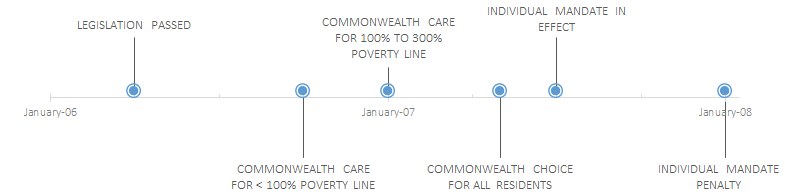
\includegraphics[width=\textwidth]{resources/timeline}
	\caption{Timeline of plans available for individual purchase and mandate requirements}
	\label{fig:reformTimeline}
\end{figure}

A net effect of the act was a drop in uninsured Massachusetts residents. The Massachusetts Health Insurance Survey is conducted in the first half of each year and asks about the current insurance status of Massachusetts residents. It suggests that the act resulted in an approximate 60\% reduction in uninsured adult residents. Figure \ref{fig:uninsuredRate} illustrates the effect by contrasting the periods before and after the law was fully implemented. 

\begin{figure}[H]
	\centering
	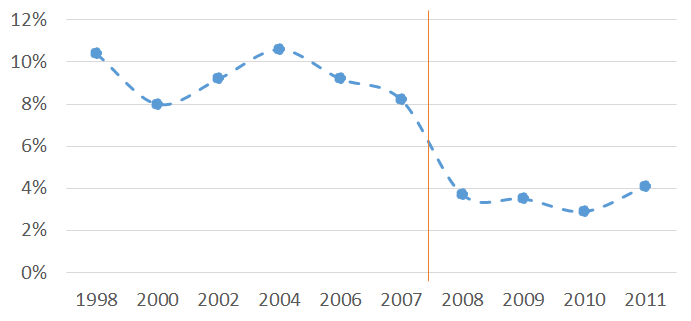
\includegraphics[scale=0.6]{resources/uninsured}
	\caption{Percent of Massachusetts residents uninsured between the ages of 19 to 64}
	\label{fig:uninsuredRate}
\end{figure}

From an entrepreneurial standpoint, we view the act as having improved the health insurance marketplace for self-employed residents. We are agnostic to the mechanism. One possibility is the lower cost of insurance; Gruber \cite{gruber_mass} suggests that controlling for plans with lower benefits, the cost of individual insurance plans dropped by 20\% as a results of the reforms. Other potential mechanisms include the ability to sign up for plans with pre-existing conditions and greater confidence in keeping insurance conditional on becoming sick. We use the period starting in 2008 as the treatment period for the shock since the law's main effect of lowering the uninsured rate was observed in 2008. 

Simultaneity is a concern in our setting. We can imagine there exists both a supply of individuals willing to become an entrepreneur as well as a demand for entrepreneurs in the form of opportunities for entrepreneurship. We assume the health care reforms have a minor impact on opportunities for entrepreneurship outside of the health care industry in our analysis. The assumption would be false if for example the health reform freed up enough disposable income to significantly increase spending on restaurants. Holding our assumption enables us to identify how the health care law changes the supply of entrepreneurship. 

\begin{comment}

Another concern is whether the stable unit treatment value assumption (SUTVA) holds. It can fail if for example entrepreneurs moved from Rhode Island to Massachusetts to take advantage of the health reform. If this occurs, we expect our results to be biased upwards. We believe our use of synthetic controls based on counties across the US helps isolates us from violations since any mobility . 

\end{comment}

\section{Theoretical Motivation}
\label{sec:model}

\subsection{Aggregate Effect}

We will use this empirical context to test four propositions. First, building on Gruber and Madrain \cite{gm2002}, consider a compensating differential model of a worker that currently has health care through their job but expects to be unable to attain health care as an entrepreneur. Utility is a function of both returns to an activity and a binary indicator of health insurance coverage. We can imagine the returns to an activity being dependent on tangible characteristics such as wages as well as less tangible ones such as job satisfaction. Workers stay at the firm as long as the return to employment $w$ and the return to entrepreneurship $r$ as such that
$$U(w,1) \ge U(r,0)$$

If there is a shock that creates a market for non-group health insurance at utility cost $c$, the worker will stay are long as
$$U(w,1) \ge \max\{U(r,0),U(r-c,1)\}$$

This should shift some mass of workers to become entrepreneurs as long as some workers value health insurance more than the cost on the non-group health market and for those workers
$$U(w,1) < U(r-c,1)$$

So this model would predict that the health-care shock increases entrepreneurship. 

\textbf{Proposition 1:} 
Improving access to health-care should increase entrepreneurship. 

\subsection{Tax Heterogeneity}

However, the reform in Massachusetts also involved changes to government expenditure. In 2013, 30\% of the Massachusetts budget was spent on the Mass Health \cite{masshealth} subsidy program. This may have affected the expected return $r$ to self-employment conditional on creating a successful firm if for example entrepreneurs believed the subsidies would eventually be paid for by a higher progressive tax on earnings.

This could be viewed as a mitigating the effect of the shock on self-employment. Now workers will leave if the utility change in taxes $t$ is such that

$$U(w,1) < U(r-t-c,1)$$

These expectations should affect incentives to create non-profit firms differently than for-profit firms. In the above model utility is decreasing in taxes so non-profit firms should gain more from the reform so we should see a heterogenous effect of the shock across these two types of firms.  

\textbf{Proposition 2:} 
The health care reform package should cause a relatively larger increase in non-profit firms than for-profit firms. 

Note we are assuming that the utility cost of health insurance, $c$, is the same for non-profit and for-profit entrepreneurs.  

\subsection{Capital Heterogeneity}

Our next proposition considers another form of industry based heterogeneity. Suppose a potential entrepreneur is considering to start a new venture. Conditional on having an opportunity, factors such as ability to attract complementary talent \cite{stuartSorensen} can impact the decision to execute the venture. We can model the probability of starting a firm as the probability of getting an opportunity that fits the constraints binding the entrepreneur. 

Suppose two such constraints are the capital required to start the firm and access to healthcare  outside of current employment. An opportunity can vary on both dimensions. Some ideas can of course require more capital to execute than others. Additionally, some ideas could be worked on without leaving existing employment. For example, survey data suggests half of all software developers create applications outside of their formal employment \cite{evans}. Also, the constraints are likely to vary by individual. Individuals vary in their social networks which can influence access to capital \cite{uzzi}. A potential entrepreneur may be relatively less constrained by health care if her spouse's employer provided health insurance for their family. 

\textbf{Proposition 3:} 
Suppose opportunities to start low capital firms are at least as common as high capital firms. Then improving access to healthcare should increase the probability of starting a low capital firm relative to a high capital firm. Equality or a negative difference between the low and high capital groups suggests low capital opportunities are strongly constrained outside of access to health care. 

\textbf{Proof:}
See Appendix A for a formal statement of the proposition, its required assumptions and its proof. 

The intuition behind Proposition 3 can be conveyed in the single entrepreneur case using a visualization of the space of potential opportunities. Suppose an entrepreneur has a level $\alpha_i$ of healthcare and level $\beta_i$ of capital to start with. The entrepreneur can then execute opportunities that require at most those levels of resources. The shaded region in Figure \ref{fig:ideaSpace} represents the space of opportunities executable by the entrepreneur. If we think of the healthcare reform as shifting level $\alpha_i$ to $\alpha_i'$, the striped region's set of opportunities also become feasible. Note that only opportunities with resource requirements lower than $\beta_i$ are affected by the shift in resource $\alpha$. As long as there is not a larger mass of potential opportunities that require high capital than low capital, when we sum across all individual entrepreneurs we should see more executed opportunities with low capital than high capital. 

\begin{figure}[H]
	\centering
	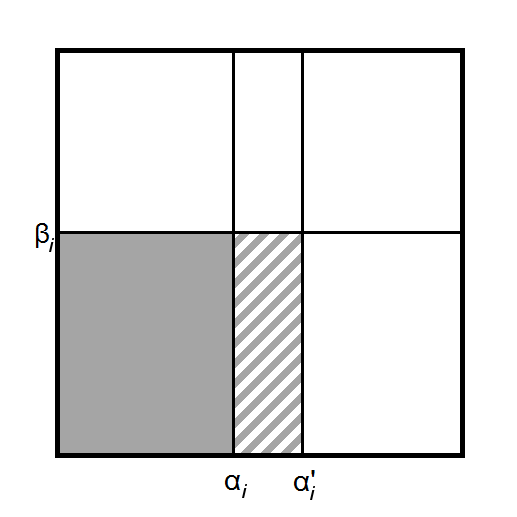
\includegraphics[scale=0.5]{resources/Prop1}
	\caption{Subset of opportunity space executable by agent $i$ with resources $(\alpha_i,\beta_i)$ versus$(\alpha_i', \beta_i)$.}
	\label{fig:ideaSpace}
\end{figure}

Our last proposition describes the relative short and long term affect of a health care shock. 

\textbf{Proposition 4:} The relative increase in low versus high capital firms should attenuate over time. 

\textbf{Proof:} See Appendix A for a formal statement and proof

This follows from entrepreneurs having any memory of past opportunities. Immediately after the shock, opportunities in Figure \ref{fig:ideaSpace}'s striped region that occurred to the entrepreneur in the current time period as well as prior periods become feasible. In future periods, feasible opportunities are only drawn from the new ideas generated by the entrepreneur that period.


\section{Data Sources}
\label{sec:data}


We measure our outcome variable of entrepreneurship with two different US Census data sets. First we focus on self-employment as measured in the American Community Survey (ACS). The ACS surveys households for employment status and provides information on self-employment rates on a county basis. Although this self-employment data lacks the industry classification necessary for main findings, it connects well with previous research that estimated the impact of health reform on self-employment rates. 

To test our hypothesis related to industry characteristics, we use the Nonemployer Statistics (NS) series also from the US Census. The NS is based on tax filings and includes self-employed individuals as well incorporated businesses and partnerships that lack employees. 

\begin{comment}

Our second source of data is the Census Country Business Patterns (CBP). The CBP is an annual series based on the Census Business Register, a dataset of US firms that is continuously updated using multiple methods including surveys and tax reporting. The CBP provides country level information on for example the industry, sales and employee count of establishments. It excludes businesses with no paid employees. As shown in Figure \ref{fig:firm_est}, establishments closely track firms. Although we are primarily interested in new firm creation, the census does not publicly provide firm level data at the industry level per county. We use establishments of 1 to 4 employees (small establishments) as a proxy for entrepreneurial firms. 

\begin{figure}[H]
	\centering
	\includegraphics[scale=0.6]{resources/firm_est_MA.eps}
	\caption{Number of firms and establishments in Massachusetts with 1 to 4 employees}
	\label{fig:firm_est}
\end{figure}

Our third source of data is the Nonemployer Statistics series. The NS is based on tax filings. It includes self-employed individuals as well incorporated businesses and partnerships that lack employees. 

\end{comment}

Both of our data sources suffer from being measurements of net rather than gross values. For example, if  we do not obverse a change in number self-employed individuals over a period of time, this does not necessarily mean no new enterprises were created. No change happens when the rate of establishment entrance equals the rate of firm establishment. Exit and entrance are also definitional; a previously existent firm that hired its first worker would be listed as a exit in the NS data one year but an entrant in a following year if that worker was later laid off. Unfortunately we were not able to find a satisfactory public data set with gross establishment or firm numbers. However we think any change in the rate of entrepreneurship will still manifest in our dataset. To illustrate, figure \ref{fig:construct} shows how the number of nonemployers changes in construction, a traditionally cyclical industry. We see a rise during the boom period of mid-2000 followed by a fall after the 2008 recession. 

\begin{figure}[H]
	\centering
	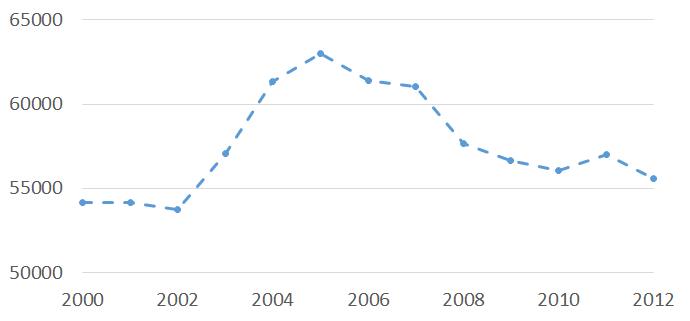
\includegraphics[scale=0.6]{resources/construction.eps}
	\caption{Number of nonemployers in the MA construction industry}
	\label{fig:construct}
\end{figure}

Table \ref{tab:basic} provides summary statistics for our variables of interest in Massachusetts and other New England states from 2000 to 2012. To reduce potential endogeneity we remove firms in the health care industry from our dataset. The rest of New England is approximately similar to Massachusetts in size and establishment characteristics although Massachusetts is more urban than the rest of New England. 

\begin{table}[H]
	\centering
	\caption{Summary statistics for Massachusetts and other New England states}
	\begin{tabular}{lrr} \hline \hline
& Massachusetts  & Other New England  \\  \hline
Population &   6,431,559 &    7,847,646 \\
Percent Urban &        91.09\% &        60.91\% \\
Percent Uninsured &        13.50\% &        13.74\% \\
Percent Aged 20 to 24 &         6.40\% &         5.94\% \\
Percent of Households with Children &        30.60\% &        31.68\% \\
\hline \textbf{Self-Employment} & & \\
Number &      210,684 &      311,317\\
Percent of Population &       3.28\% &       4.01\% \\
Yearly Change in Percent of Population &         -0.01\% &         -0.02\% \\
\hline \textbf{Non-employers} & & \\
Number &      423,846 &      572,954\\
Percent of Population &       6.39 \% &       7.15 \% \\
Yearly Change in Percent of Population &          0.06 \% &          0.07 \% \\
 \hline \hline \end{tabular}

	\label{tab:basic}
\end{table}

In order to measure the effect of the health care reform on entrepreneurship, ideally we would want to measure change in probability that an individual becomes an entrepreneur. Given that our dataset that lacks observations of individuals, we focus on the changes in our variables of interest. For our first proposition, we measure this as the change in percentage of self-employed people per county ($Change_{ct}$). For our other propositions, we measure the change in non-employed establishments per million people in each county ($Change_{cit}$) by industry. The large number of 4 digit NAICS classifications causes us to use the million people denominator; simple percentages would lead to coefficients that become cumbersome to read. 

\begin{comment}

This differs from the more common usage of percentage of self-employed in a given sub-population. We do not think the percentage approach is applicable in our case because we expand beyond self-employed workers to consider the count of firms; we believe the number of firms per million people has a more intuitive interpretation than the percentage of firms in a population of people.


\begin{figure}[H]
	\centering
	\includegraphics[scale=.75]{resources/naics_summary}
	\caption{Average yearly change in number of small establishments per 1M residents}
\end{figure}

Figure 4 shows by county the change in number of small establishments per 1M residents both before and after the treatment. We see a similar pattern across Massachusetts counties and the rest of New England. 

\begin{figure}[H]
	\centering
	\includegraphics[scale=.75]{resources/county_summary}
	\caption{Average yearly change in number of small establishments per 1M residents}
\end{figure}


Additionally we use data from the Census Survey of Business Owners (SBO) to understand characteristics of entrepreneurial firms. Table 3 provides for example the number of firm owners indicating no startup capital was required to start the business.  It includes all non-farm businesses with revenue greater than \$1000 per year that file with the IRS. Unlike the CBP, the SBO includes firms with no employees.

\begin{flushleft}
\scalebox{.9}{
\begin{tabular}{|c|l|r|}
\hline
NAICS & Industry & No funding\\
\hline
61 & Educational Services &	19.2\%\\
71 & Arts, Entertainment, and Recreation  &	17.9\%\\
22 & Utilities	 & 16.8\%\\
55 & Management of Companies and Enterprises &	15.4\%\\
52 & Finance and Insurance &	14.5\%\\
54 & Professional, Scientific and Technical Services &	12.1\%\\
21 & Mining, Quarrying, and Oil and Gas Extraction & 	11.9\%\\
23 & Construction &	11.8\%\\
51 & Information &	11.8\%\\
62 & Health Care and Social Assistance &	11.8\%\\
53 & Real Estate and Rental and Leasing &	11.6\%\\
56 & Administrative, Support, Waste Management, Remediation Services &	11.0\%\\
11 & Agriculture, Forestry, Fishing and Hunting &	10.2\%\\
42 & Wholesale Trade &	10.1\%\\
48-49 & Transportation and Warehousing &	9.3\%\\
31-33 & Manufacturing &	9.1\%\\
81 & Other Services, except Public Administration &	8.7\%\\
44-45 & Retail Trade &	6.9\%\\
72 & Accommodation and Food Services &	5.3\%\\
\hline
\end{tabular}
}
\end{flushleft}

Finally, we use the 2012 Economic Census Industry Series for information about the concentration of non-profits per industry. The data classifies firms by whether they are exempt from federal income tax in some service industries. We exclude the subset of industries relating to health care services.

\end{comment}

\section{Empirical Approach}
\label{sec:regression}

\subsection{Overall Impact}

Proposition 1 suggests we should see an increase in entrepreneurial activity after the health care reform. To test this prediction, we first apply a difference in differences approach with counties in Massachusetts as the treatment group and various controls. If the reform improved the return to entrepreneurship for some workers, our treatment indicator should be positive. 
\begin{align}
Change_{cst} = \alpha_c + \zeta_s + \delta_t + \beta \, \mathbf{1}\{\text{county in MA}\} \cdot \mathbf{1}\{\text{year > 2007}\} + \epsilon_{cst}
\end{align}

Here $Change_{cst}$ represents the change in our variable of interest per million residents in year $t$ and county $c$ of state $s$. The model includes fixed effects for year ($\delta$), county ($\alpha$) and state ($\zeta$).

Our first control consists of counties in New England outside of Massachusetts. We define New England as Connecticut, Maine, New Hampshire, Rhode Island, Vermont and Massachusetts. This helps account for broad regional shocks such as recessions that affect all of New England. 

For a more targeted approach, we use border matching as our second control. Here our treatment group consists of Massachusetts counties that share a border with another state. This pulls out the cities of Boston and Cambridge. Our control group consists of counties in Connecticut, New Hampshire, Rhode Island, Vermont and New York that border Massachusetts. We would expect this method to help ensure our control and treatment groups are similar if geographically close counties  have for example more similar economic activity than distant counties. 

Finally we employ a synthetic control method drawing on counties across all US states other than Massachusetts. Our approach mirrors the procedure used in Abadie et al. \cite{abadie} although we slightly modify their source code to better account for rounding errors in our specific use case. For each county in Massachusetts we generate a synthetic pair as a control. We first prune the matching pool by removing counties that strongly differ from the Massachusetts county in either level of urbanization, uninsured rate, population age, or the frequency of children in a household. We then assign weights to the pruned set of counties in order to minimize the difference in our outcome variable between control and treatment before our shock. This has the benefit of removing any pre-trend from our natural experiment as seen in Figure \ref{fig:state_contrast}. The downside is that the matching is done algorithmically and may produce counterintuitive controls. In our case the procedure yielded arguably valid results; self-employment rates in Boston (Suffolk County, MA) before 2008 most closely matched a combination the counties for Ann Arbor, MI (57\% weight), Lexington, KY (25\% weight) and other various counties across the US. 

\begin{figure}[H]
	\centering
	\begin{subfigure}[b]{0.495\textwidth}
		\includegraphics[width=\textwidth]{tmp/graphpoint_diff_se_pop_new_england}
		\caption{Other New England states as control}
	\end{subfigure}
		\begin{subfigure}[b]{0.495\textwidth}
		\includegraphics[width=\textwidth]{tmp/graphpoint_diff_se_pop_synthetic}
		\caption{Synthetic control}
	\end{subfigure}
	\caption{Treatment Effect for Self-Employed Individuals}
	\label{fig:state_contrast}
\end{figure}

\subsection{Non-profit Heterogeneity}

Proposition 2 predicts that non-profits were more strongly impacted by the health care reform since there is no long term cost of increased taxes that balances the short term benefit of health care access. To test this prediction, we use Economic Census data that provides information about the number of tax paying and tax-exempt establishments at the 4 digit NAICS code industry level for a subset of industries.  

Our first specification restricts our observations to counties in Massachusetts. For each of our industries we use the percentage of the industry's firms that were excluded from federal taxes as a measure of treatment intensity. 
\begin{comment}

We interpret our coefficient of interest as a lower bound estimate of the health care shock impact. It is a lower bound because for-profit industries may have also benefited and we are measuring the difference between the two sets of industries.

\begin{align}
Change_{cit} = \alpha_c + \gamma_i + \delta_t + \beta \, \mathbf{1}\{\text{non-profit industry}\} \cdot \mathbf{1}\{\text{year > 2007}\} + \epsilon_{ct}
\end{align}

\begin{align}
Change_{cit} = & \; \gamma_i \cdot \alpha_c + \gamma_i \cdot \delta_t +  \alpha_c \cdot \delta_t \nonumber   \\
& + \beta \, \mathbf{1}\{\text{non-profit industry}\} \cdot \mathbf{1}\{\text{year > 2007}\}  \cdot \mathbf{1}\{\text{county in  MA}\} \nonumber  \\
& + \epsilon_{ict}
\end{align}

\end{comment}
\begin{align}
Change_{cit} = \alpha_c + \gamma_i + \delta_t + \beta \times \{\text{\% of industry non-profit}\} \cdot \mathbf{1}\{\text{year > 2007}\} + \epsilon_{ct}
\end{align}

Here $Change_{cit}$ represents the number of net new establishments created per million residents in year $t$, county $c$ and industry $i$. The model includes fixed effects for year ($\delta$), county ($\alpha$) and industry ($\gamma$). Although our observations are based on NAICS codes at the 4 digit level, we apply fixed effect $\gamma$ at the 2 digit NAICS code level in order to have a manageable number of coefficients to estimate given the constraints of our data set. Since our self-employment data set lacks industry information we only apply model (2) to our non-employer data set. 

Model (2) leaves open the possibility of another shock happening at the same time that also differentially affected non-profit industries. The results would be invalid if for example the 2008 recession was relatively milder for non-profit firms than for for-profit firms. To control for this, we extend our approach to a triple difference model which should account for shocks that both affected Massachusetts and our synthetic control. 
\begin{align}
Change_{cit} = & \; \gamma_i \cdot \alpha_c + \gamma_i \cdot \delta_t +  \alpha_c \cdot \delta_t \nonumber   \\
& + \beta  \times \{\text{\% of industry non-profit}\} \cdot \mathbf{1}\{\text{year > 2007}\}  \cdot \mathbf{1}\{\text{county in  MA}\} \nonumber  \\
& + \epsilon_{ict}
\end{align}



\subsection{Capital Requirement Heterogeneity}

Proposition 3 states that as long as opportunities for low capital entrepreneurship are at least as prevalent as opportunities for high capital entrepreneurship, we should see that the health insurance shock increased low capital entrepreneurship relative to high capital entrepreneurship. We first test this proposition using model (4) within Massachusetts. 
\begin{align}
Change_{cit} =  \alpha_c + \gamma_i+ \delta_t + \beta \, \mathbf{1}\{\text{low capital industry}\} \cdot \mathbf{1}\{\text{year >= 2008}\} + \epsilon_{ict}
\end{align}

As with our non-profit analysis we continue to define industry by 4 digit NAICS codes. We use the Survey of Business Owners (SBO) Public Use Microdata Sample (PUMS) from 2007 to determine which industries have low capital requirements. Since the SBO PUMS data only reports on 2 digit NAICS codes, we calculate the percentage of businesses that required less than \$1000 of startup capital for each 2 digit NAICS code and match the 2 digit NAICS codes with our 4 digit industry codes. We consider industries above the middle of the range of percentages as low capital industries. We avoid treatment intensity in this case in contrast to our non-profit approach because we have insufficient industry granularity at the 2 digit NAICS code level. The PUMS data provides the capital requirements by employment size so we customize our calculation of low capital industries for firms with no employees. 

Model (4) leaves open the possibility of another shock happening at the same time that also differentially affected low capital industries. We therefore include the triple difference model (5). 
\begin{align}
Change_{cit} = & \; \gamma_i \cdot \alpha_c + \gamma_i \cdot \delta_t +  \alpha_c \cdot \delta_t \nonumber   \\
& + \beta \, \mathbf{1}\{\text{low capital industry}\} \cdot \mathbf{1}\{\text{year >= 2008}\}  \cdot \mathbf{1}\{\text{county in MA}\} \nonumber  \\
& + \epsilon_{cit}
\end{align}

Finally for Proposition 4 we modify the difference in difference to see if the short term treatment results was stronger than the long term treatment results in model (6) with a corresponding triple differences estimator in model (7). 
\begin{align}
Change_{cit} & =  \alpha_c + \gamma_i+ \delta_t  \nonumber + \beta_{0} \, \mathbf{1}\{\text{low capital industry}\} \cdot \mathbf{1}\{\text{year in initial shock}\} \nonumber \\
& + \beta_{1} \, \mathbf{1}\{\text{low capital industry}\} \cdot \mathbf{1}\{\text{year > initial shock}\} + \epsilon_{ict} \\
Change_{cit} & =  \; \gamma_i \cdot \alpha_c + \gamma_i \cdot \delta_t +  \alpha_c \cdot \delta_t \nonumber   \\
& + \beta_{0} \, \mathbf{1}\{\text{low capital industry}\} \cdot \mathbf{1}\{\text{year in initial shock}\}  \cdot \mathbf{1}\{\text{county in MA}\} \nonumber  \\
& + \beta_{1} \, \mathbf{1}\{\text{low capital industry}\} \cdot \mathbf{1}\{\text{year > initial shock}\}  \cdot \mathbf{1}\{\text{county in MA}\} \nonumber  \\
& + \epsilon_{cit}
\end{align}

Unfortunately our theory does not provide a clear mechanism for determining what is short term versus long term. Some opportunities made possible by the health care shock could be executed on immediately while others may require careful planning over a significant amount of time. We use Figure \ref{fig:ddd} as a guide. It plots the model (5) residuals over time. We observe there is an attenuation after three years of treatment for non-employers. We think the most useful test of Proposition 4 would be to have the initial shock be considered as years 2008 to 2009. If we do not see a statistical significant drop in this case, then we can rule out Proposition 4 with some confidence. 

\begin{figure}[H]
	\centering
	\includegraphics[width=0.6\textwidth]{tmp/graphpoint_capital_ne}
	\caption{Treatment Effect of triple difference model with New England as control}
	\label{fig:ddd}
\end{figure}

\begin{comment}
\begin{figure}[H]
	\centering
	\begin{subfigure}[b]{0.495\textwidth}
		\includegraphics[width=\textwidth]{resources/graphpoint_diff_ne_pop_ddd_synth}
		\caption{Non-Employers}
	\end{subfigure}
		\begin{subfigure}[b]{0.495\textwidth}
		\includegraphics[width=\textwidth]{resources/graphpoint_diff_em_pop_ddd_synth}
		\caption{Small businesses}
	\end{subfigure}
	\caption{Treatment Effect of triple difference model with synthetic control}
\end{figure}
\end{comment}

\subsection{Inference}

Fixed effects with errors clustered by state is the usual approach to inference when dealing with state wide shocks. However as pointed out by Donald and Lang \cite{donald}, inference with a small number of cluster groups can suffer from large bias. In our New England control specification we only have 5 groups. We also have limited observations per group; each New England state just has 11 counties on average so the two-step approach suggested by Donald and Lang does not apply. In addition, our shock only applies to a single state cluster leading to a singular covariance matrix under our modeling specification; see Appendix B for an illustration with a simple linear model. 

To address these concerns, we use a Monte-Carlo simulation described in Appendix C to test various inference approaches conditional on the properties of our dataset. As a result, we report confidence intervals based on Huber-White errors. 

\section{Findings}
\label{sec:results}

\subsection{Importance of Control Group}

Table \ref{tab:control} summarizes our first finding as a test of Proposition 1. We run the difference in difference model (1) against the yearly percentage change in self employed population. Over our period of interest, about 3.29\% of Massachusetts' population was unincorporated, self employed individuals. Our column 1 result suggests the percentage of self-employed residents increased by 0.08 per year as a result of health care reform, for an overall increase of 0.4\% by the end of our period of interest. This result compares well to the Becker and Tuzemen \cite{tuzemen} result of 0.6\% which measured the impact of the same shock on self employment using an IV approach on aggregate state data. 

However we find the magnitude of our results to be sensitive to the control group in use. Column 2 uses the border county procedure to attempt a closer match between our treatment and control groups. Column 3 uses the synthetic control group process. Both results in similar standard errors but magnitudes that are not distinguishable from zero. 
\begin{center}
	\begin{table}[H]
		\centering
			\caption{Diff-in-diff estimator of yearly percentage change in self-employment} 
		{
\def\sym#1{\ifmmode^{#1}\else\(^{#1}\)\fi}
\begin{tabular}{l*{3}{c}}
\hline\hline
          &\multicolumn{1}{c}{(1)}&\multicolumn{1}{c}{(2)}&\multicolumn{1}{c}{(3)}\\
\hline
Massachusetts $\times$ Post 2007&    0.075** &    0.063   &    0.040   \\
          &  (0.030)   &  (0.037)   &  (0.031)   \\
[1em]
Year FE   &      Yes   &      Yes   &      Yes   \\
[1em]
State FE  &      Yes   &      Yes   &      Yes   \\
[1em]
County FE &      Yes   &      Yes   &      Yes   \\
\hline
\(N\)     &      804   &      264   &      336   \\
\(R^{2}\) &    0.050   &    0.136   &    0.109   \\
Control   &New England   &Border Counties   &Synthetic   \\
Weight    &Population   &Population   &Population   \\
\hline\hline
\multicolumn{4}{l}{\footnotesize Standard errors in parentheses}\\
\multicolumn{4}{l}{\footnotesize * p<0.10, ** p<0.05, *** p<0.01}\\
\multicolumn{4}{l}{\footnotesize Diff-in-diff model of health care reform from 2000 to 2012 with Massachusetts treated after 2007. }\\
\multicolumn{4}{l}{\footnotesize Maine, Connecticut, Vermont, Rhode Island and New Hampshire used as controls in column (1). }\\
\multicolumn{4}{l}{\footnotesize Column (3) uses a synthetic control model that matches each Massachuetts county pre-trend against}\\
\multicolumn{4}{l}{\footnotesize \space US counties with similar income, age, urban and insurance rate characteristics. }\\
\end{tabular}
}
	
		\label{tab:control}
	\end{table}		
\end{center}
\begin{comment}
Diff-in-diff model of health care reform from 2000 to 2012 with Massachusetts treated after 2007. Maine, Connecticut, Vermont, Rhode Island and New Hampshire used as controls in column (1). Column (2) restricts the dataset to counties that border other states across Massachusetts, Connecticut, Vermont, Rhode Island, New Hampshire and New York. Column (3) uses a synthetic control model that matches each Massachuetts county pre-trend against US counties with similar income, age, urban and insurance rate characteristics. 
\end{comment}

We interpret these findings to mean any possible effect our shock had on self-employment is likely to be too small to detect using the publicly available census data on individuals. We believe the sensitivity to control explains why the Becker and Tuzemen \cite{tuzemen} results differ from the Heim and Lurie results \cite{heimLurie}. 

\subsection{Long Run Tax Impact}

Table \ref{tab:nonprofit} shows our results testing Proposition 2 claim that non-profit firm creation should increase faster than for-profit firm creation. Column 1's results from running model (2) suggests a noticeable effect, which remains once we apply the triple difference specified in model (3) with the New England and synthetic controls. Although our estimate under border control loses its significance, we interpret our overall results as supporting Proposition 2. The magnitude of our observed effect is large. Our estimate suggests that an industry composed only of non-profits would gain about 52 new firms per million people each year relative to an industry composed only of for-profit firms. To contrast, our dataset shows on average 13 new firms were created per million people each year for a typical industry. 

\begin{table}[H]
	\centering
	\caption{Impact of health reform on non-profit non-employers}
	{
\def\sym#1{\ifmmode^{#1}\else\(^{#1}\)\fi}
\begin{tabular}{l*{4}{c}}
\hline\hline
          &\multicolumn{1}{c}{(1)}&\multicolumn{1}{c}{(2)}&\multicolumn{1}{c}{(3)}&\multicolumn{1}{c}{(4)}\\
\hline
\% Non-profit $\times$ Post 2007&   42.565***&            &            &            \\
          &  (9.203)   &            &            &            \\
MA $\times$ \% Non-profit $\times$ Post 2007&            &   52.015***&   20.728   &   52.550***\\
          &            & (14.387)   & (18.712)   & (12.941)   \\
County $\times$ Year FE &       No   &      Yes   &      Yes   &      Yes   \\
Industry $\times$ Year FE &       No   &      Yes   &      Yes   &      Yes   \\
County $\times$ Industry FE &       No   &      Yes   &      Yes   &      Yes   \\
Year FE   &      Yes   &       No   &       No   &       No   \\
County FE &      Yes   &       No   &       No   &       No   \\
State FE  &      Yes   &       No   &       No   &       No   \\
Industry FE &      Yes   &       No   &       No   &       No   \\
\hline
\(N\)     &     3288   &    10560   &     4236   &     6384   \\
\(R^{2}\) &    0.019   &    0.143   &    0.121   &    0.131   \\
Control   &Within MA   &New England   &Border Counties   &    Synth   \\
\hline\hline
\multicolumn{5}{l}{\footnotesize Standard errors in parentheses}\\
\multicolumn{5}{l}{\footnotesize * p<0.10, ** p<0.05, *** p<0.01}\\
\multicolumn{5}{l}{\footnotesize Column (1) is a diff-in-diff model of non-employers per million people in Massachusetts from  }\\ 
\multicolumn{5}{l}{\footnotesize \space 2000 to 2012 with treatment after 2007 and treatment intensity equal to percentage of non-profit}\\ 
\multicolumn{5}{l}{\footnotesize \space firms within industry.}\\ 
\multicolumn{5}{l}{\footnotesize Non-profit industries defined by 4 digit NAICS codes where over half of firms were tax-exempt }\\
\multicolumn{5}{l}{\footnotesize  \space according to 2007 Economic Census data.}\\
\multicolumn{5}{l}{\footnotesize Maine, Connecticut, Vermont, Rhode Island and New Hampshire used as controls in column (2) }\\
\multicolumn{5}{l}{\footnotesize \space under triple diff model. }\\
\multicolumn{5}{l}{\footnotesize Column (3) restricts the dataset to counties that border other states across Massachusetts, }\\
\multicolumn{5}{l}{\footnotesize \space Connecticut, Vermont, Rhode Island, New Hampshire and New York. }\\
\multicolumn{5}{l}{\footnotesize Column (4) uses a synthetic control model that matches each Massachuetts industry by county }\\
\multicolumn{5}{l}{\footnotesize \space pre-trend against US counties with similar income, age, urban and insurance rate characteristics. }\\
\end{tabular}
}

	\label{tab:nonprofit}
\end{table}

\begin{comment}

\multicolumn{4}{l}{\footnotesize Column (1) is a diff-in-diff model of non-employers per million people in Massachusetts from  }\\ 
\multicolumn{4}{l}{\footnotesize \space 2000 to 2012 with treatment after 2007 and treatment intensity equal to percentage of non-profit firms within industry.}\\ 
\multicolumn{4}{l}{\footnotesize Non-profit industries defined by 4 digit NAICS codes where over half of firms were tax-exempt }\\
\multicolumn{4}{l}{\footnotesize  \space according to 2007 Economic Census data.}\\
\multicolumn{4}{l}{\footnotesize Maine, Connecticut, Vermont, Rhode Island and New Hampshire used as controls in column (2) }\\
\multicolumn{4}{l}{\footnotesize \space under triple diff model. }\\
\multicolumn{4}{l}{\footnotesize Column (3) restricts the dataset to counties that border other states across Massachusetts, }\\
\multicolumn{4}{l}{\footnotesize \space Connecticut, Vermont, Rhode Island, New Hampshire and New York. }\\
\multicolumn{4}{l}{\footnotesize Column (4) uses a synthetic control model that matches each Massachuetts industry by county }\\
\multicolumn{4}{l}{\footnotesize \space pre-trend against US counties with similar income, age, urban and insurance rate characteristics. }\\

\begin{table}[H]
	\centering
	{
\def\sym#1{\ifmmode^{#1}\else\(^{#1}\)\fi}
\begin{tabular}{l*{4}{c}}
\hline\hline
          &\multicolumn{1}{c}{(1)}&\multicolumn{1}{c}{(2)}&\multicolumn{1}{c}{(3)}&\multicolumn{1}{c}{(4)}\\
\hline
\% Non-profit $\times$ Post 2007&   42.565***&            &            &            \\
          &  (9.203)   &            &            &            \\
MA $\times$ \% Non-profit $\times$ Post 2007&            &   52.015***&   20.728   &   52.550***\\
          &            & (14.387)   & (18.712)   & (12.941)   \\
County $\times$ Year FE &       No   &      Yes   &      Yes   &      Yes   \\
Industry $\times$ Year FE &       No   &      Yes   &      Yes   &      Yes   \\
County $\times$ Industry FE &       No   &      Yes   &      Yes   &      Yes   \\
Year FE   &      Yes   &       No   &       No   &       No   \\
County FE &      Yes   &       No   &       No   &       No   \\
State FE  &      Yes   &       No   &       No   &       No   \\
Industry FE &      Yes   &       No   &       No   &       No   \\
\hline
\(N\)     &     3288   &    10560   &     4236   &     6384   \\
\(R^{2}\) &    0.019   &    0.143   &    0.121   &    0.131   \\
Control   &Within MA   &New England   &Border Counties   &    Synth   \\
\hline\hline
\multicolumn{5}{l}{\footnotesize Standard errors in parentheses}\\
\multicolumn{5}{l}{\footnotesize * p<0.10, ** p<0.05, *** p<0.01}\\
\multicolumn{5}{l}{\footnotesize Column (1) is a diff-in-diff model of non-employers per million people in Massachusetts from  }\\ 
\multicolumn{5}{l}{\footnotesize \space 2000 to 2012 with treatment after 2007 and treatment intensity equal to percentage of non-profit}\\ 
\multicolumn{5}{l}{\footnotesize \space firms within industry.}\\ 
\multicolumn{5}{l}{\footnotesize Non-profit industries defined by 4 digit NAICS codes where over half of firms were tax-exempt }\\
\multicolumn{5}{l}{\footnotesize  \space according to 2007 Economic Census data.}\\
\multicolumn{5}{l}{\footnotesize Maine, Connecticut, Vermont, Rhode Island and New Hampshire used as controls in column (2) }\\
\multicolumn{5}{l}{\footnotesize \space under triple diff model. }\\
\multicolumn{5}{l}{\footnotesize Column (3) restricts the dataset to counties that border other states across Massachusetts, }\\
\multicolumn{5}{l}{\footnotesize \space Connecticut, Vermont, Rhode Island, New Hampshire and New York. }\\
\multicolumn{5}{l}{\footnotesize Column (4) uses a synthetic control model that matches each Massachuetts industry by county }\\
\multicolumn{5}{l}{\footnotesize \space pre-trend against US counties with similar income, age, urban and insurance rate characteristics. }\\
\end{tabular}
}

	\caption{Impact of health reform on non-profit entrepreneurship}
\end{table}

\end{comment}

\subsection{Entrepreneurship Unconstrained by Health Care}

Table \ref{tab:capital_ne} summarizes the results of testing Proposition 3 using our dataset of non-employing establishments. Column 1 uses the difference in difference estimator of model (4) to show overall low capital industries grew slower than high capital industries after our shock. However as with our non-profit analysis, the result attenuates to be indistinguishable from zero once we apply our various control groups under the triple difference model (5). 

We next turn to Proposition 4 which provides us with more statistical accuracy if the shock's impact was short lived. Column 2 of table \ref{tab:capital_ne_ext} shows a significant effect under the triple difference model of model (7) with other New England states as a control. The result is not robust to other controls as we see in Column 3 and Column 4. 

Note that our point estimates based on both Proposition 3 and 4 are negative, regardless of significance. Our theory predicts a negative or zero result if opportunities for low capital firms were somehow constrained by other factors. In other words, our results suggest that entrepreneurship in Massachusetts is being significantly constrained by something other than the lack access to health insurance. 

\begin{table}[H]
	\centering
	\caption{Impact of health reform on low capital industries}
	{
\def\sym#1{\ifmmode^{#1}\else\(^{#1}\)\fi}
\begin{tabular}{l*{4}{c}}
\hline\hline
          &\multicolumn{1}{c}{(1)}&\multicolumn{1}{c}{(2)}&\multicolumn{1}{c}{(3)}&\multicolumn{1}{c}{(4)}\\
\hline
Low Capital $\times$ Post 2007&  -41.768***&            &            &            \\
          & (11.716)   &            &            &            \\
MA $\times$ Low Capital $\times$ Post 2007&            &  -39.330***&  -28.867***&  -20.084***\\
          &            & (11.981)   &  (8.286)   &  (7.772)   \\
County $\times$ Year FE &       No   &      Yes   &      Yes   &      Yes   \\
Industry $\times$ Year FE &       No   &      Yes   &      Yes   &      Yes   \\
County $\times$ Industry FE &       No   &      Yes   &      Yes   &      Yes   \\
Year FE   &      Yes   &       No   &       No   &       No   \\
County FE &      Yes   &       No   &       No   &       No   \\
State FE  &      Yes   &       No   &       No   &       No   \\
Industry FE &      Yes   &       No   &       No   &       No   \\
\hline
\(N\)     &     8676   &    26040   &    11124   &    16824   \\
\(R^{2}\) &    0.023   &    0.391   &    0.601   &    0.649   \\
Control   &Within MA   &New England   &Border Counties   &    Synth   \\
\hline\hline
\multicolumn{5}{l}{\footnotesize Standard errors in parentheses}\\
\multicolumn{5}{l}{\footnotesize * p<0.10, ** p<0.05, *** p<0.01}\\
\multicolumn{5}{l}{\footnotesize Column (1) is a diff-in-diff model of non-employers per million people in Massachusetts from  }\\ 
\multicolumn{5}{l}{\footnotesize \space 2000 to 2012 with treatment after 2007 and treatment intensity equal to percentage of non-profit}\\ 
\multicolumn{5}{l}{\footnotesize \space firms within industry.}\\ 
\multicolumn{5}{l}{\footnotesize Low capital industries defined by 4 digit NAICS industries with high percentage of firms }\\
\multicolumn{5}{l}{\footnotesize \space requiring less \$1000 of startup capital according to Survey of Business Owners 2007 Public Use }\\
\multicolumn{5}{l}{\footnotesize \space Microdata Sample }\\
\multicolumn{5}{l}{\footnotesize Maine, Connecticut, Vermont, Rhode Island and New Hampshire used as controls in column (2) }\\
\multicolumn{5}{l}{\footnotesize \space under triple diff model. }\\
\multicolumn{5}{l}{\footnotesize Column (3) restricts the dataset to counties that border other states across Massachusetts, }\\
\multicolumn{5}{l}{\footnotesize \space Connecticut, Vermont, Rhode Island, New Hampshire and New York. }\\
\multicolumn{5}{l}{\footnotesize Column (4) uses a synthetic control model that matches each Massachuetts industry by county }\\
\multicolumn{5}{l}{\footnotesize \space pre-trend against US counties with similar income, age, urban and insurance rate characteristics. }\\
\end{tabular}
}

	\label{tab:capital_ne}
\end{table} 

\begin{comment}

\multicolumn{4}{l}{\footnotesize Column (1) is a diff-in-diff model of non-employers per million people in Massachusetts from  }\\ 
\multicolumn{4}{l}{\footnotesize \space 2000 to 2012 with treatment after 2007 and treatment intensity equal to percentage of non-profit}\\ 
\multicolumn{4}{l}{\footnotesize \space firms within industry.}\\ 
\multicolumn{4}{l}{\footnotesize Non-profit industries defined by 4 digit NAICS codes where over half of firms were tax-exempt }\\
\multicolumn{4}{l}{\footnotesize  \space according to 2007 Economic Census data.}\\
\multicolumn{4}{l}{\footnotesize Maine, Connecticut, Vermont, Rhode Island and New Hampshire used as controls in column (2) }\\
\multicolumn{4}{l}{\footnotesize \space under triple diff model. }\\
\multicolumn{4}{l}{\footnotesize Column (3) restricts the dataset to counties that border other states across Massachusetts, }\\
\multicolumn{4}{l}{\footnotesize \space Connecticut, Vermont, Rhode Island, New Hampshire and New York. }\\
\multicolumn{4}{l}{\footnotesize Column (4) uses a synthetic control model that matches each Massachuetts industry by county }\\
\multicolumn{4}{l}{\footnotesize \space pre-trend against US counties with similar income, age, urban and insurance rate characteristics. }\\

\begin{table}[H]
	\centering
	\input{resources/main_diff_ne_pop.tex}
	\caption{Impact of health reform on low capital industries}
\end{table}

\end{comment}

\begin{table}[H]
	\centering
	\caption{Initial versus long term impact of health reform on low capital industries}
	\input{tmp/capital_ext.tex}
	\label{tab:capital_ne_ext}
\end{table} 

\begin{comment}

\multicolumn{4}{l}{\footnotesize Column (1) is a diff-in-diff model of non-employers per million people in Massachusetts from  }\\ 
\multicolumn{4}{l}{\footnotesize \space 2000 to 2012 with low capital industries treated after 2007 and high capital industries as control.}\\ 
\multicolumn{4}{l}{\footnotesize Treatment broken out into initial period of 2008 to 2009 and longer term period of 2010 to 2012.}\\ 
\multicolumn{4}{l}{\footnotesize Low capital industries defined by 2 digit NAICS industries with high percentage of firms }\\
\multicolumn{4}{l}{\footnotesize \space requiring less \$1000 of startup capital according to Survey of Business Owners 2007 Public Use }\\
\multicolumn{4}{l}{\footnotesize \space Microdata Sample }\\
\multicolumn{4}{l}{\footnotesize Maine, Connecticut, Vermont, Rhode Island and New Hampshire used as controls in column (2) }\\
\multicolumn{4}{l}{\footnotesize \space under triple diff model. }\\
\multicolumn{4}{l}{\footnotesize Column (3) restricts the dataset to counties that border other states across Massachusetts, }\\
\multicolumn{4}{l}{\footnotesize \space Connecticut, Vermont, Rhode Island, New Hampshire and New York. }\\
\multicolumn{4}{l}{\footnotesize Column (4) uses a synthetic control model that matches each Massachuetts industry by county }\\
\multicolumn{4}{l}{\footnotesize \space pre-trend against US counties with similar income, age, urban and insurance rate characteristics. }\\


\begin{table}[H]
	\centering
	\input{resources/main_diff_em_pop.tex}
	\caption{Impact of health reform on low capital industries}
\end{table}

\end{comment}

\section{Conclusion}
\label{sec:conclude}

We have used the 2006 policy change in Massachusetts as a shock to better understand the relationship between entrepreneurship and access to health insurance. We have tested a number of theories suggesting entrepreneurship rates would increase overall and differentially within non-profit and low capital industries. 

Our first result was to show that previous results suggesting a positive overall relationship may have be an artifact of poor control design. Our analysis estimated a statistically significant increase in self-employment when we used the rest of New England as a control. However the significance disappeared under both a county border matching strategy and a synthetic control strategy. Many of the high tech industries clustered around the Kendell Square in Cambridge, MA may not be adequately represented in the rest of New England. These kinds of regional variations may be causing the inconsistencies in our estimates when we vary our control design. 

Our second result addresses whether the policy shock's short term benefits of improved access to health care is counterbalanced by entrepreneurial concerns of higher future taxes to pay for those benefits. Our results support this hypothesis. Previous literature  has consistently shown a negative relationship between tax rates and entrepreneurship; here we provide evidence expectations about future taxes can also change entry rates. We are however hesitant to conclude that changes in tax expectations mitigate the entrepreneurial benefits of health insurance reform. Our theoretical model assumed that the utility costs of health insurance were the same between entrepreneurs deciding to start non-profit and for-profit firms. We can imagine selection issues invaliding that assumption if for example entrepreneurs starting non-profit firms are less likely to have access to health insurance through an employed spouse. 

Our final result connects the entrepreneurial health insurance question to capital constraints. We have the unexpected finding that capital intensive industries fared better than low capital industries. Our theory shows this could only be the case if there were significantly more new opportunities in high capital industries relative to low capital industries as a result of the shock. We interpret these findings as saying activities such as freelancing that require low capital are constrained by factors other than access to health insurance. As our quoted Kendell Square entrepreneur suggests, it seems the lack of health care is not stopping entrepreneurs from pursuing their business ideas. 

Our overall contribution consists not only of the individual results themselves but also a new approach to analyze shocks to entrepreneurship. We believe using heterogeneity in new firm characteristics will be useful for entrepreneurial scholars studying health insurance as well as other potential barriers to entrepreneurship. 

\begin{comment}

Our results point the way to future research in this area. Our results may be sensitive to for example the subsidy schedule based on income implemented in Massachusetts. In addition, more precise firm creation data sources may allow us to make stronger statements about the types of industries that benefited from health care reform.


Reasons why no result is plausible: 
People will do this anyway
Cost of insurance is not covered; still expensive. 
People disuaded small sub-sample of entrepreneurs, pre-existing conditions or those with kids but no spousal insurance or access to VC funds

However 
Long and Dahlen \footnote{Long Dahlen 2014} and Long, Stockly and Nordahl \footnote{2012} show insurance rates increased primarily among low income, childless adults. Not the demographic for entrepreneurs. 

\end{comment}

\newpage

\appendix
\section*{Appendix}
\subsection*{Appendix A}

Let $\Omega$ represent the set of all possible opportunities. In each time period $t$, a potential entrepreneur $i$ makes a draw $\omega_{it} \subset \Omega$ from this set. To simplify assume each entrepreneur makes the same number of draws in each period. 

Assume that ideas can be totally ordered based on each of the factors. Let $X:\Omega\to I^n \subset \mathbb{R}^n$ be a random variable where $n$ is the number of factors that can impact the decision to start a company. For example, consider an opportunity $\omega$ to start a software company. One of the factors required might be a software developer with an advanced knowledge of computer science. The random variable would assign a real number that represents the knowledge required to the dimension $j$ of $\mathbb{R}^n$ that represents software development skill as a factor. Another opportunity $\omega'$ that requires less advanced software development would be assigned a number less than the first opportunity. 
$$X(\omega)^j > X(\omega')^j $$

Let $r_i \in I^n$ represent the resources of the entrepreneur. To continue the example, the software entrepreneur may have access through her social network to a novice software developers but no connections to more advanced developers. An opportunity is executed by the entrepreneur if all required factors can be met by the entrepreneur. 
$$r_i^j \ge X(\omega_{it})^j \; \forall j \in n$$

\begin{comment}
We call an idea \textit{unbounded} for an individual if the idea can be executed and \textit{single bounded} on dimension $k$ if
$$\alpha_i^k = X(\omega{it})^k \wedge  \alpha_i^j > X(\omega{it})^j \; \forall j \ne k \in n$$
\end{comment}

The probability of an opportunity being executed by an entrepreneur with resources $r_i$ in time $t$ is therefore 
$$Pr\left(\bigcap _{j=1}^n  r_i^j \ge X^j\right) = F_X(r)$$
Let $F_Y$ represent the distribution of entrepreneurs with resources $r$ over the space of opportunities. Then the expected number of startups generated at time $t$ is then 
\begin{align}
\mathbb{E}_{Y}[F_X(r)]=\int_{I^n} F_X(r) dF_Y(r)
\end{align}

Consider how a change in the distribution of resources for one factor impacts the rate of startup creation along another factor's dimension. For example, increasing access to healthcare might impact the rate of firm creation for ideas requiring large amounts of capital differently than ideas require low amounts of capital. Let $\alpha$ represent the factor being changed, $\beta$ the factor we are measuring a reaction to, and $\Gamma$ be the set of all other factors. Let $\beta_0$ be a specific resource level on $\beta$ we are interested in and $[\underline{I_\beta}, \beta_0]$ the set of all resource levels that are equal to or less than $\beta_0$. We can write the total number of startups (6) that fall within that resource level as
\begin{align*}
& \int_{I^n} F_X(r) dF_Y(r)\\
= & \int_{I^n} \int_{\underline{I^n}}^{r} dF_X(s) dF_Y(r)\\
= & \int_{I^n} \int_{s}^{\overline{I^n}}  dF_Y(r) dF_X(s) \\
= &  \int_{I_{\Gamma}} \int_{I_{\alpha,\beta}} \int_{s}^{\overline{I^n}}  dF_Y(r)dF_{X_{\alpha,\beta}}(a,b|U)
 dF_{X_{\Gamma}}(U)\\
= &  \int_{I_{\Gamma}} \int_{I_{\alpha,\beta}} \int_{U}^{\overline{I_\Gamma}} \int_{a,b}^{\overline{I_{\alpha,\beta}}} dF_{Y_{\alpha,\beta}}(s,t|V)dF_{Y_\Gamma}(V) dF_{X_{\alpha,\beta}}(a,b|U) dF_{X_{\Gamma}}(U)\\
= &  \int_{I_{\Gamma}} \int_{U}^{\overline{I_\Gamma}} \int_{I_{\alpha,\beta}} \int_{a,b}^{\overline{I_{\alpha,\beta}}} dF_{Y_{\alpha,\beta}}(s,t|V) dF_{X_{\alpha,\beta}}(a,b|U) dF_{Y_\Gamma}(V) dF_{X_{\Gamma}}(U)\\
= &  \int_{I_{\Gamma}} \int_{U}^{\overline{I_\Gamma}} \int_{I_{\beta}} \int_{I_{\alpha}} \int_{b}^{\overline{I_{\beta}}} \int_{a}^{\overline{I_{\alpha}}} dF_{Y_{\alpha,\beta}}(s,t|V) dF_{X_{\alpha,\beta}}(a,b|U) dF_{Y_\Gamma}(V) dF_{X_{\Gamma}}(U)\\
\implies S(\beta_0) = & \int_{I_{\Gamma}} \int_{U}^{\overline{I_\Gamma}} \int_{\underline{I_\beta}}^{\beta_0} \int_{I_{\alpha}} \int_{b}^{\overline{I_{\beta}}} \int_{a}^{\overline{I_{\alpha}}} dF_{Y_{\alpha,\beta}}(s,t|V) dF_{X_{\alpha,\beta}}(a,b|U) dF_{Y_\Gamma}(V) dF_{X_{\Gamma}}(U)
\end{align*}
Define a function $h$ that maps the conditional distribution entrepreneurs on resource $\alpha$ and a value $\beta_0$ to the rate of new enterprise creation at $\beta_0$ conditional on $\Gamma$.
\begin{align*}
h(G_{Y_\alpha},\beta_0|\Gamma) = \int_{I_{\alpha}} \int_{\beta_0}^{\overline{I_{\beta}}} \int_{a}^{\overline{I_{\alpha}}} dG_{Y_{\alpha}}(s|t) dF_{Y_{\beta}}(t) dF_{X_{\alpha,\beta}}(a,\beta_0) = \left. \frac{\partial S (\beta_0|\Gamma)}{\partial \beta} \right|_{G_{Y_{\alpha}}=F_{Y_{\alpha}}}
\end{align*}

Finally, use first order stochastic dominance to define a partial order on the set of all distributions for $G_{Y_\alpha}$. 

\textbf{Proposition 3:} 
The function $h$ has increasing differences in $G_{Y_\alpha}$ and $-\beta_0$ if $dF_{X_{\alpha,\beta}}$ is non-increasing in $\beta$. 

\textbf{Proof:}
Let $G'_{Y_\alpha}\mathop{\ge}_{\text{FOSD}} G_{Y_\alpha}$ and $\beta_0' \ge \beta_0$. Then $h$ has increasing differences in $G_{Y_\alpha}$ and $-\beta_0$ if and only if:
\begin{align*}
& h(G'_{Y_\alpha},\beta_0|\Gamma) - h(G'_{Y_\alpha},\beta_0'|\Gamma) \ge h(G_{Y_\alpha},\beta_0|\Gamma) - h(G_{Y_\alpha},\beta_0'|\Gamma)\\
\iff & h(G'_{Y_\alpha},\beta_0|\Gamma) - h(G_{Y_\alpha},\beta_0|\Gamma) \ge h(G'_{Y_\alpha},\beta_0'|\Gamma) - h(G_{Y_\alpha},\beta_0'|\Gamma)\\
\iff & \int_{I_{\alpha}} \int_{\beta_0}^{\overline{I_{\beta}}} \int_{a}^{\overline{I_{\alpha}}} dG'_{Y_{\alpha}}(s|t) dF_{Y_{\beta}}(t) dF_{X_{\alpha,\beta}}(a,\beta_0) \\ 
& - \int_{I_{\alpha}} \int_{\beta_0}^{\overline{I_{\beta}}} \int_{a}^{\overline{I_{\alpha}}} dG_{Y_{\alpha}}(s|t) dF_{Y_{\beta}}(t) dF_{X_{\alpha,\beta}}(a,\beta_0) \\
& \ge \int_{I_{\alpha}} \int_{\beta_0'}^{\overline{I_{\beta}}} \int_{a}^{\overline{I_{\alpha}}} dG'_{Y_{\alpha}}(s|t) dF_{Y_{\beta}}(t) dF_{X_{\alpha,\beta}}(a,\beta_0') \\
& - \int_{I_{\alpha}} \int_{\beta_0'}^{\overline{I_{\beta}}} \int_{a}^{\overline{I_{\alpha}}} dG_{Y_{\alpha}}(s|t) dF_{Y_{\beta_0}}(t) dF_{X_{\alpha,\beta}}(a,\beta_0')\\
\iff & \int_{I_{\alpha}} \int_{\beta_0}^{\overline{I_{\beta}}} \int_{a}^{\overline{I_{\alpha}}} (dG'_{Y_{\alpha}}(s|t) - dG_{Y_{\alpha}}(s|t)) dF_{Y_{\beta}}(t) dF_{X_{\alpha,\beta}}(a,\beta_0) \\ 
& \ge \int_{I_{\alpha}} \int_{\beta_0'}^{\overline{I_{\beta}}} \int_{a}^{\overline{I_{\alpha}}} (dG'_{Y_{\alpha}}(s|t) - dG_{Y_{\alpha}}(s|t)) dF_{Y_{\beta}}(t) dF_{X_{\alpha,\beta}}(a,\beta_0')\\
\iff & \int_{I_{\alpha}} \int_{\beta_0}^{\overline{I_{\beta}}} (1-G'_{Y_{\alpha}}(a|t)) - (1-G_{Y_{\alpha}}(a|t)) dF_{Y_{\beta}}(t) dF_{X_{\alpha,\beta}}(a,\beta_0) \\ 
& \ge \int_{I_{\alpha}} \int_{\beta_0'}^{\overline{I_{\beta}}} (1-G'_{Y_{\alpha}}(a|t)) - (1-G_{Y_{\alpha}}(a|t)) dF_{Y_{\beta}}(t) dF_{X_{\alpha,\beta}}(a,\beta_0') \\ 
\iff & \int_{I_{\alpha}} \int_{\beta_0}^{\overline{I_{\beta}}} (G_{Y_{\alpha}}(a|t) - G'_{Y_{\alpha}}(a|t)) dF_{Y_{\beta}}(t) dF_{X_{\alpha,\beta}}(a,\beta_0) \\ 
& \ge \int_{I_{\alpha}} \int_{\beta_0'}^{\overline{I_{\beta}}} (G_{Y_{\alpha}}(a|t) - G'_{Y_{\alpha}}(a|t)) dF_{Y_{\beta}}(t) dF_{X_{\alpha,\beta}}(a,\beta_0')
\end{align*}
$G'_{Y_\alpha} \mathop{\ge}_{\text{FOSD}} G_{Y_\alpha}$ implies $G_{Y_{\alpha}}(a|t) - G'_{Y_{\alpha}}(a|t)$ is non-negative, so 
\begin{align*}
\int_{I_{\alpha}} \int_{\beta_0}^{\overline{I_{\beta}}} (G_{Y_{\alpha}}(a|t) - G'_{Y_{\alpha}}(a|t)) dF_{Y_{\beta}}(t) dF_{X_{\alpha,\beta}}(a,\beta_0)
\end{align*}
is also non-negative since events can only have non-negative measure. Since $dF_{X_{\alpha,\beta}}$ is non-increasing in $\beta$, we have: 
\begin{align*}
& \int_{I_{\alpha}} \int_{\beta_0}^{\overline{I_{\beta}}} (G_{Y_{\alpha}}(a|t) - G'_{Y_{\alpha}}(a|t)) dF_{Y_{\beta}}(t) dF_{X_{\alpha,\beta}}(a,\beta_0)\\
& \ge \int_{I_{\alpha}} \int_{\beta_0}^{\overline{I_{\beta}}} (G_{Y_{\alpha}}(a|t) - G'_{Y_{\alpha}}(a|t)) dF_{Y_{\beta}}(t) dF_{X_{\alpha,\beta}}(a,\beta_0')
\end{align*}
So the proof would be completed if
\begin{align*}
& \int_{I_{\alpha}} \int_{\beta_0}^{\overline{I_{\beta}}} (G_{Y_{\alpha}}(a|t) - G'_{Y_{\alpha}}(a|t)) dF_{Y_{\beta}}(t) dF_{X_{\alpha,\beta}}(a,\beta_0') \\
&  \ge  \int_{I_{\alpha}} \int_{\beta_0'}^{\overline{I_{\beta}}} (G_{Y_{\alpha}}(a|t) - G'_{Y_{\alpha}}(a|t)) dF_{Y_{\beta}}(t) dF_{X_{\alpha,\beta}}(a,\beta_0')\\
\iff & \int_{I_{\alpha}} \int_{\beta_0}^{\beta_0'} (G_{Y_{\alpha}}(a|t) - G'_{Y_{\alpha}}(a|t)) dF_{Y_{\beta}}(t) dF_{X_{\alpha,\beta}}(a,\beta_0') \ge 0\\
\end{align*}
Which again is true from $G'_{Y_\alpha} \mathop{\ge}_{\text{FOSD}} G_{Y_\alpha}$ and the restriction to non-negative measures. $\Box$ \\

This modeling requires shocks to cause first order stochastically dominated shifts in access to a resource. The health care act fulfills this requirement if it only weakly increases the probability that an individual has enough access to health insurance to execute a given opportunity. It cannot for example change the distribution of access to capital or the distribution of ideas. We believe this is the case as long as we exclude firms in the health care sector from our analysis since the shock could have created new opportunities for health entrepreneurship.  

The non-increasing condition can be interpreted as saying that we should not see more ideas for startups as the required amount of resources increases. Following our example, in general there should not be more opportunities that require high capital than ideas that require lower capital. If this condition fails to hold then we will obverse an attenuation of the modeled effect. 

Note that the required FOSD shift in $\alpha$ is allowed to be conditional on the level of resource $\beta$ possessed by the entrepreneur. In our example we can imagine entrepreneurs with access to high levels of capital to be less effected by the health care act than entrepreneurs with access to low levels of capital.  

Next, consider how an increase in the distribution of $F_{Y_\alpha}$ impacts ideas from previous periods if those ideas are retained by the entrepreneur. Each period $T$'s expected number of startups becomes
\begin{align}
\mathbb{E}^T_Y[F_{X}] = \mathbb{E}_{Y_T}[F_{X}] + \sum_{t=0}^{T-1} max(0,\mathbb{E}_{Y_T}[F_{X}] - max(\mathbb{E}_{Y_i}[F_{X}] \forall i \in T{-}1,\dots,t)))
\end{align}

\textbf{Proposition 4:} If in any three consecutive periods $t=0,1,2$
\begin{enumerate}[(a)]
\item $F_{Y_\alpha,t=1} \mathop{\ge}_{\text{FOSD}} F_{Y_\alpha,t=0} $
\item $F_{Y_\alpha,t=1} = F_{Y_\alpha,t=2} $
\item $F_{Y_-\alpha|\alpha,t=0} = F_{Y_-\alpha|\alpha,t=1} =F_{Y_-\alpha|\alpha,t=2}$
\end{enumerate}
then
\begin{enumerate}[(a)]
\setcounter{enumi}{3}
\item $\mathbb{E}_{Y}[F_{Y_\alpha,t=1}] \ge \mathbb{E}_{Y}[F_{Y_\alpha,t=2}]$
\item $\mathbb{E}_{Y}[F_{Y_\alpha,t=2}] \ge \mathbb{E}_{Y}[F_{Y_\alpha,t=0}]$
\end{enumerate}

\textbf{Proof:} (d) follows from (2) and the expectation properties of first order stochastic dominance. (e) follows also from the properties of first order stochastic dominance.

\subsection*{Appendix B}

Suppose we have $N$ individuals $i$ spread across $M$ groups $g$. Linear regression of observed outcomes $Y_i$ against a vector of independent variables $X_i$ solves a system of equations for $\beta$. 
$$ \hat{\beta} = \underset{\beta}{\arg \min} \; \sum_{i=1}^{N} (Y_i - X_i' \beta)^2 \implies \sum_{g=1}^{M} \sum_{i \in g} X_i(Y_i - X_i' \hat{\beta}) = 0$$

In addition, suppose we have a treatment indicator variable $X_i^t$ with a corresponding coefficient $\beta^t$ and the treatment is one for just a single group $g^t$. We can rewrite the system of equations and note the sum of its residuals for the group $g^t$ equals zero by construction. 
\begin{align*}
& \sum_{g=1}^{M} \sum_{i \in g} \begin{bmatrix}
X_i^{-t} \\  X_i^t 
\end{bmatrix}(Y_i - \begin{bmatrix}
X_i^{-t} \\  X_i^t 
\end{bmatrix}' \begin{bmatrix}
\hat{\beta}^{-t} \\ \hat{\beta}^t 
\end{bmatrix}) = \\  & \; \sum_{g\ne g^t}^{M} \sum_{i \in g} \begin{bmatrix}
X_i^{-t} \\  0 
\end{bmatrix}(Y_i - \begin{bmatrix}
X_i^{-t} \\  0 
\end{bmatrix}' \begin{bmatrix}
\hat{\beta}^{-t} \\ \hat{\beta}^t 
\end{bmatrix}) + \sum_{i \in g^t} \begin{bmatrix}
X_i^{-t} \\  1 
\end{bmatrix}(Y_i - \begin{bmatrix}
X_i^{-t} \\  1 
\end{bmatrix}' \begin{bmatrix}
\hat{\beta}^{-t} \\ \hat{\beta}^t 
\end{bmatrix}) = 0 \\
& \implies \sum_{i \in g^t} (1) 
(Y_i - \begin{bmatrix}
X_i^{-t} \\  1 
\end{bmatrix}' \begin{bmatrix}
\hat{\beta}^{-t} \\ \hat{\beta}^t 
\end{bmatrix}) = 0
\end{align*}

The covariance matrix for clustered standard errors take the form:
$$ \hat{V} \propto (X'X)^{-1} \left( \sum_{g=1}^{M} \sum_{i \in g} \left(\begin{bmatrix}
X_i^{-t} \\  X_i^t 
\end{bmatrix}(Y_i - \begin{bmatrix}
X_i^{-t} \\  X_i^t 
\end{bmatrix}' \begin{bmatrix}
\hat{\beta}^{-t} \\ \hat{\beta}^t 
\end{bmatrix})\right)' \begin{bmatrix}
X_i^{-t} \\  X_i^t 
\end{bmatrix}(Y_i - \begin{bmatrix}
X_i^{-t} \\  X_i^t 
\end{bmatrix}' \begin{bmatrix}
\hat{\beta}^{-t} \\ \hat{\beta}^t 
\end{bmatrix})  \right)  (X'X)^{-1}$$ 

We observe that in the inner summation when $g \ne g^t$ we are adding matrices with zero's in the last column and row since $X^t_i$ will be zero. When $g = g^t$, from above we know the group's residual is zero by construction so we have a zero matrix. Therefore the inner matrix must be singular which implies the covariance matrix is also singular. 

\subsection*{Appendix C}

In order to construct confidence intervals given the issues with our small group size, we first use a monte-carlo simulation to test various approaches. Our data generating process is based on a modifided version of model (1) allowing for auto-correlated residuals and state level shocks. 
\begin{comment}
\begin{align}
Change_{sct} & = \alpha_c + \gamma_s + \delta_t + \beta \, \mathbf{1}\{\text{county in MA}\} \cdot \mathbf{1}\{\text{year > 2007}\} + \xi_{sct} \\
\xi_{sct} & = 
\begin{cases}\rho_{sc} \, \xi_{sc(t-1)} + (1-\rho_{sc}) \epsilon_{sct} &\mbox{if } t > 1 \nonumber \\ 
\epsilon_{sct}  & \mbox{if } t = 1. \end{cases}\\
\epsilon_{sct} & = \mu_{st} + \upsilon_{sct}
\end{align}
Here $\rho$ is a random variable with distribution $\mathcal{F}$, $\mu$ is a random variable with distribution $\mathcal{G}$ and $\upsilon$ is a random variable with distribution $\mathcal{H}$. We estimate $\hat{\rho}_{sc}$ for each county in New England by regressing $Change_{sct}$ against $Change_{sc(t-1)}$ in our self-employed dataset. $\mathcal{F}$ is then approximated by taking uniform draws from the set of $\hat{\rho}_{sc}$'s. We group the residuals from the $\hat{\rho}_{sc}$ estimation by state and divide them by $1/(1-\hat{\rho}_{sc})$ to generate a set of $\hat{\epsilon}_{sct}$ values. We use the mean of $\hat{\epsilon}_{sct}$ values grouped by state and year to produce a set of $\hat{\mu}_{st}$ values that once standardized appropriate $\mathcal{G}$. Then $\hat{\epsilon}_{sct}$ minus the corresponding $\hat{\mu}_{st}$ values produce a set of $\hat{\upsilon}_{sct}$ draws that once standardized approximate $\mathcal{H}$.
\end{comment}
\begin{align}
Change_{sct} & = \alpha_c + \gamma_s + \delta_t + \beta \, \mathbf{1}\{\text{county in MA}\} \cdot \mathbf{1}\{\text{year > 2007}\} + \xi_{sct} \\
\xi_{sct} & = 
\begin{cases}\rho_{sc} \, \xi_{sc(t-1)} + (1-\rho_{sc}) \epsilon_{sct} &\mbox{if } t > 1 \nonumber \\ 
\epsilon_{sct}  & \mbox{if } t = 1. \end{cases}
\end{align}
Here $\rho$ is a random variable with distribution $\mathcal{F}$ and $\epsilon$ is a random variable with distribution $\mathcal{G}_s$ that varies by state. We estimate $\hat{\rho}_{sc}$ for each county in New England by regressing $Change_{sct}$ against $Change_{sc(t-1)}$ in our self-employed dataset. $\mathcal{F}$ is then approximated by taking uniform draws from the set of $\hat{\rho}_{sc}$'s. We group the residuals from the $\hat{\rho}_{sc}$ estimation by state and divide them by $1/(1-\hat{\rho}_{sc})$ to similarly create approximations for the $\mathcal{G}_s$ set. 

In order to test for Type 1 error, we set $\beta$ to zero in equation 8, simulate the data and drop our first year's observations since they lack an auto-correlated term. To test Type 2 error, we set $\beta$ equal to a third of the standard deviation of $Change_{sct}$. Through experiment we determined this value produced sufficient variation between our inference methods for comparison. We run fixed effects regressions under homeostatic, robust, stated clustered and auto-regressive error assumptions. We also calculate Newey-West errors with a 3 year and we use a 2 step block bootstrap method with re-sampling of counties within states using the scaling correction suggested by Rao and Wu \cite{rao}. 

Table \ref{tab:mc} presents the results. We see that fixed effects under AR(1) assumptions does the best overall. However the assumption of an AR(1) process was baked into our data generating process through our functional form; it may not accurately reflect our observed data. We therefore select robust inference as preferred for our dataset since robust errors do not show excessive Type 1 error and it performs slightly better than our bootstrap procedure on Type 2 error.

\begin{table}[H]
	\centering
	\caption{Monte Carlo Simulation of Type 1 and 2 Errors}
	\begin{tabular}{lrrrr} \hline \hline
		Specification &(1) & (2) & (3) & (4)  \\  
		\hline \textbf{Simulation Parameters} & & & & \\
		States &   5 &    2 & 5 & 2\\
		Counties per State &        10 &        100 & 10 & 100\\
		Years of Observations &        12 &        12 & 12 & 12 \\
		Treatment Value &        0 &        0 & $\sigma_{Y}/3$ & $\sigma_{Y}/3$\\
		Draws &       200 & 200 & 200 & 200\\
		\hline \multicolumn{5}{l}{\textbf{Percent Rejecting Null Hypothesis}} \\
		Fixed Effects OLS &      20\% &      40\%& 49\%& \textbf{96}\%\\
		FE Huber-White &       \textbf{2\%} &       \textbf{2\%}& 44\%& 67\%\\
		FE Clustered by State &         29\% &         50\%& 62\% & 51\%\\
		FE AR(1) Process &         \textbf{2\%} &         \textbf{0\%}& 28\%& \textbf{98\%}\\
		Panel Newey-West &         9\% &         18\%& 59\% & 84\%\\
		Block Bootstrap &        \textbf{2\%} &         \textbf{2\%}& 33\%& 67\%\\
		\hline \hline 
		\multicolumn{5}{l}{\footnotesize 95\% confidence interval used to test null hypothesis. Bold  }\\
		\multicolumn{5}{l}{\footnotesize indicates values that either do not over-reject null when true }\\
		\multicolumn{5}{l}{\footnotesize  treatment is zero or do not under-reject null when true  }\\
		\multicolumn{5}{l}{\footnotesize treatment is non-zero. }\\
	\end{tabular}	
	\label{tab:mc}
\end{table}


\begin{comment}

\subsection*{Appendix B}

\begin{figure}[H]
	\centering
	\includegraphics[scale=.8]{resources/NAICS_99.eps}
	\caption{Total establishments with 1 to 4 employees in Massachusetts by NAICS code}
\end{figure}

In Figure 4 we see the industry classified as NAICS 99 as changing drastically versus the other industries in the data set. NAICS 99 generally refers to unclassified firms. 

\subsection*{Appendix C}

Calculating the kernel density over the entire range of Kickstarter goals provides unsatisfactory results due to extreme values. There is for example a project with a stated goal of \$100,000,000, far higher than any funded project on Kickstarter. Of the top ten funded projects on Kickstarter, the highest project goal was just \$2,000,000. \\

\begin{tabular}{|l | r| r|}
	\hline
	Project & Goal & Funding \\
	\hline
	Pebble Time	& \$500,000  & \$20,338,986\\
	Coolest Cooler & \$50,000  & \$13,285,226\\
	Pebble & \$100,000 & \$10,266,845\\
	Exploding Kittens & \$10,000 & \$8,782,571\\
	OUYA & \$950,000  & \$8,596,474\\
	Pono Music & \$800,000  & \$6,225,354\\
	Veronica Mars Movie Project & \$2,000,000  & \$5,702,153\\
	Reading Rainbow & \$1,000,000  & \$5,408,916\\
	Torment & \$900,000  & \$4,188,927\\
	\hline
\end{tabular} \\

We therefore omit projects with goals \$5,000,000 or greater from the density estimate; these projects are abnormally high relative to what is realistic on Kickstarter. They likely reflect aspirational goals that go beyond the true capital requirements of the inventor's idea. 

\end{comment}

\newpage

\begin{thebibliography}{99}

\bibitem{abadie}
Abadie, Alberto, Alexis Diamond, and Jens Hainmueller. ``Synthetic control methods for comparative case studies: Estimating the effect of California’s tobacco control program.'' Journal of the American Statistical Association 105.490 (2010).

\bibitem{bailey}
Bailey, James B., ``Health Insurance and the Supply of Entrepreneurs: New Evidence from the Affordable Care Act's Dependent Coverage Mandate'' (March 7, 2013). 

\bibitem{tuzemen}
Becker, Thealexa and Didem T\"{u}zemen. ``Health Care Reform and Self-Employment: Evidence From Massachusetts.'' \emph{Federal Reserve Bank of Kansas City Research Working Paper} 14-16, 2014.

\bibitem{cullen}
Cullen, Julie Berry, and Roger H. Gordon. ``Taxes and entrepreneurial risk-taking: Theory and evidence for the US.'' Journal of Public Economics 91.7 (2007): 1479-1505.

\bibitem{darin}
Da Rin, Marco, Marina Di Giacomo, and Alessandro Sembenelli. ``Entrepreneurship, firm entry, and the taxation of corporate income: Evidence from Europe.'' Journal of public economics 95.9 (2011): 1048-1066.

\bibitem{djankov}
Djankov, Simeon, et al. ``The effect of corporate taxes on investment and entrepreneurship.'' No. w13756. National Bureau of Economic Research, 2008.

\bibitem{donald}
Donald, Stephen G., and Kevin Lang. "Inference with difference-in-differences and other panel data." The review of Economics and Statistics 89.2 (2007): 221-233.

\bibitem{evans}
Evans, David S., and Boyan Jovanovic. ``An estimated model of entrepreneurial choice under liquidity constraints.'' The Journal of Political Economy (1989): 808-827.

\bibitem{fairlie_health}
Fairlie, Robert W., Kanika Kapur, and Susan Gates. "Is employer-based health insurance a barrier to entrepreneurship?." Journal of Health Economics 30.1 (2011): 146-162.

\bibitem{garthwaite}
Garthwaite, Craig, Tal Gross, and Matthew J. Notowidigdo. ``Public Health Insurance, Labor Supply, and Employment Lock.'' \emph{The Quarterly Journal of Economics} 129.2 (2014): 653-696.

\bibitem{gentry}
Gentry, William M., and R. Glenn Hubbard. ``Tax policy and entrepreneurial entry.'' American Economic Review (2000): 283-287.

\bibitem{gruber_mass}
Gruber, Jonathan. ``Massachusetts points the way to successful health care reform.'' \emph{Journal of Policy Analysis and Management} 30.1 (2011): 184-192.

\bibitem{gruberMadrian}
Gruber, Jonathan, and Brigitte C. Madrian. ``Health insurance availability and the retirement decision.'' No. w4469. \emph{National Bureau of Economic Research}, 1993.

\bibitem{gm2002}
Gruber, Jonathan, and Brigitte C. Madrian. ``Health Insurance, Labor Supply, and Job Mobility.'' Health Policy and the Uninsured (2004): 97.

\bibitem{haltiwanger}
Haltiwanger, John, Ron S. Jarmin, and Javier Miranda. ``Who creates jobs? Small versus large versus young.'' Review of Economics and Statistics 95.2 (2013): 347-361.

\bibitem{kaiser}
Henry J. Kaiser Family Foundation ``How accessible is Individual Health Insurance for consumers in less-than-perfect health?'' June 2001

\bibitem{heimLurie}
Heim, Bradley T., and Ithai Z. Lurie. ``Does health reform affect self-employment? Evidence from Massachusetts.'' \emph{Small Business Economics} (2014): 1-14.

\bibitem{holtz_capital}
Holtz-Eakin, Douglas, David Joulfaian, and Harvey S. Rosen. ``Entrepreneurial decisions and liquidity constraints.'' The Rand Journal of Economics 25.2 (1994): 334.

\bibitem{holtz_health}
Holtz-Eakin, Douglas, John R. Penrod, and Harvey S. Rosen. ``Health insurance and the supply of entrepreneurs.'' Journal of Public Economics 62.1 (1996): 209-235.

\bibitem{hurst}
Hurst, Erik, and Annamaria Lusardi. ``Liquidity constraints, household wealth, and entrepreneurship.'' Journal of political Economy 112.2 (2004): 319-347.

\bibitem{npr}
Knox, Richard. ``Romney's Mission: Massachusetts Health Care.'' \emph{National Public Radio} 8 (2006).

\bibitem{madrian}
Madrian, Brigitte C. ``Employment-Based Health Insurance and Job Mobility: Is There Evidence ofJob-Lock?.'' No. w4476. National Bureau of Economic Research, 1993.

\bibitem{masshealth}
Massachusetts Medical Policy Institute. ``MassHealth: The Basics.'' Rep. Apr. 2014. 8 May 2014 

\bibitem{miller_er}
Miller, Sarah. ``The effect of insurance on emergency room visits: an analysis of the 2006 Massachusetts health reform.'' Journal of Public Economics 96.11 (2012): 893-908.

\bibitem{olds}
Olds, Gareth ``Entrepreneurship and Public Health Insurance.'' May 2014. Working Paper

\bibitem{heritage}
Owcharenko, Nina, and Robert Moffit. ``The Massachusetts Health Plan: Lessons for the States.'' \emph{The Heritage Foundation}. 18 June 2006. Web. 27 Apr. 2015.

\bibitem{pauly}
Pauly, Mark V., and Robert D. Lieberthal. ``How risky is individual health insurance?.'' Health Affairs 27.3 (2008): w242-w249.

\bibitem{rao}
Rao, Jon NK, and C. F. J. Wu. ``Resampling inference with complex survey data.'' Journal of the American Statistical Association 83.401 (1988): 231-241.

\bibitem{census}
Smith, Jessica C., Carla Medalia ``Health Insurance in the United States: 2013.'' Current Population Reports. U.S. Census Bureau. September 2014. P60-250

\bibitem{stuartSorensen}
Stuart, Toby E., and Olav Sorenson. ``Social networks and entrepreneurship.'' \emph{Handbook of entrepreneurship research}. Springer US, 2005. 233-252.

\bibitem{sullivan}
Sullivan, Andrew. ``Obama's Meep Meep On Healthcare.'' Web log post. \emph{The Dish}. 16 Apr. 2014. 8 May 2014 

\bibitem{bisweek}
Symonds, William and Gleckman, Howard.  ``The Health-Care Crisis: States Are Rushing In.'' \emph{Business Week}. Bloomberg, 27 Nov. 2005. Web. 27 Apr. 2015.

\bibitem{toussaint}
Toussaint, Rull James, et al. ``The effect of the Massachusetts healthcare reform on the uninsured rate of the orthopaedic trauma population.'' The Journal of Bone \& Joint Surgery 96.16 (2014): e141.

\bibitem{uzzi}
Uzzi, Brian. ``Embeddedness in the making of financial capital: How social relations and networks benefit firms seeking financing.'' \emph{American Sociological Review} (1999): 481-505.

\bibitem{wellington}
Wellington, Alison J. "Health insurance coverage and entrepreneurship." Contemporary Economic Policy 19.4 (2001): 465-478.

\begin{comment}


\bibitem{acharya}
Acharya, Viral, and Krishnamurthy Subramanian, 2009, Bankruptcy codes and innovation, \emph{Review of Financial Studies} 22, 4949-4988.

\bibitem{kaufman}
Atkinson, Robert D., Scott Andes. 2010 ``The 2010 State New Economy Index: Benchmarking Economic Transformation in the States'' The Information Technology and Innovation Foundation, Kauffman Foundation


\bibitem{bhide}
Bhide, Amar. \emph{The origin and evolution of new businesses}. New York: Oxford UP, 2000.

\bibitem{bezos}
Bezos, Jeff. ``2013 Letter to Shareholders.'' Letter to Amazon shareholders. 10 Apr. 2014.

\bibitem{burton}
Burton,M.D., J. B. S{\o}rensen, C.M. Beckman. 2002. ``Coming from good stock: Career histories and new venture formation.'' M. Lounsbury, ed. \emph{Research in the Sociology of Organizations}, Vol. 19. Emerald Publishing, Bingley, UK, 229-262.

\bibitem{ericsonPakes}
Ericson, Richard, and Ariel Pakes. ``Markov-Perfect Industry Dynamics: A Framework for Empirical Work.'' \emph{The Review of Economic Studies} 62.1 (1995): 53.

\bibitem{fairlie}
Fairlie, Robert W. ``The personal computer and entrepreneurship.'' \emph{Management Science} 52.2 (2006): 187-203.

\bibitem{fairlieKarlanZinman}
Fairlie, Robert W., Dean Karlan, and Jonathan Zinman. ``Behind the GATE Experiment: Evidence on Effects of and Rationales for Subsidized Entrepreneurship Training.'' No. w17804. \emph{National Bureau of Economic Research}, 2012.


\bibitem{gompers}
Gompers, P., J. Lerner, D. Scharfstein. 2005. Entrepreneurial spawning: Public corporations and the genesis of new ventures, 1986 to 1999. \emph{J. Finance} 60(2) 577-614.

\bibitem{gruber1997}
Gruber, Jonathan. ``The Incidence of Payroll Taxation: Evidence from Chile.'' \emph{Journal of Labor Economics} 15.3 pt 2 (1997).

\bibitem{hopenhayn}
Hopenhayn, Hugo A. ``Entry, exit, and firm dynamics in long run equilibrium.'' \emph{Econometrica} (1992): 1127-1150.

\bibitem{evans}
Hurtado, Steven. ``Over Half of North American Software Developers are Moonlighting.'' \emph{Evans Data Corporation}. Nov 2012. Web. 27 Apr. 2015

\bibitem{jovanovic}
Jovanovic, Boyan. ``Selection and the Evolution of Industry.'' \emph{Econometrica} 50.3 (1982): 649.

\bibitem{klepper}
Klepper, Steven. ``Entry, exit, growth, and innovation over the product life cycle.'' \emph{American Economic Review} (1996): 562-583.

\bibitem{sommers}
Sommers, Benjamin D., Sharon K. Long, and Katherine Baicker. ``Changes in mortality after Massachusetts health care reform: a quasi-experimental study.'' Annals of internal medicine 160.9 (2014): 585-593.



\end{comment}







\begin{comment}

% <http://bluecrossmafoundation.org/sites/default/files/download/publication/PDF%20National%20comparisons%20chartpack%20june%202012.pdf/>. 


\bibitem{himmelstein}
Himmelstein, David U., Deborah Thorne, and Steffie Woolhandler. ``Medical Bankruptcy in Massachusetts: Has Health Reform Made a Difference?'' The American Journal of Medicine 124 (2011): 224-28.

\bibitem{nvca}
National Venture Captial Association. ``Q3 2014 Regional Data: Investments by State'' http://nvca.org/research/venture-investment/

\bibitem{sorensen}
Sorensen, J. B., and M. A. Fassiotto. ``Organizations as Fonts of Entrepreneurship.'' \emph{Organization Science} 22 (2011): 1322-331.


\bibitem{miller}
Miller, Sarah. ``The impact of the Massachusetts health care reform on health care use among children.'' \emph{The American Economic Review} 102.3 (2012): 502-507.

\bibitem{roy}
Roy, Andrew Donald. ``Some thoughts on the distribution of earnings.'' \emph{Oxford economic papers} 3.2 (1951): 135-146.


\bibitem{scheuer}
Scheuer, Florian. ``Entrepreneurial Taxation with Endogenous Entry.'' \emph{American Economic Journal: Economic Policy} 6.2 (2014): 126-63.

\bibitem{schumpeter}
Schumpeter, Joseph A. \emph{Capitalism, socialism, and democracy}. New York: Harper, 1950. 

\bibitem{sorensenSorensen}
Sorensen, Jesper B., and Olav Sorenson. ``From conception to birth: Opportunity perception and resource mobilization in entrepreneurship.'' \emph{Advances in Strategic Management} 20 (2003): 89-117.


\end{comment}




\begin{comment}

http://dish.andrewsullivan.com/2014/04/16/obamas-meep-meep-on-health-care


\bibitem{businessweek}
Symonds, William C. ``In Massachusetts, Health Care for All?'' Bloomberg Business Week. Bloomberg, 03 Apr. 2006. Web. 26 Jan. 2015.

\bibitem{wooldridgeBook}
Wooldridge, J. M.  2002.  Econometric Analysis of Cross Section and Panel Data.  Cambridge, MA: MIT Press.

\bibitem{census}
http://www.census.gov/prod/2008pubs/p60-235.pdf

Insured if covered by any kind of health insurance for all or part of the previous year

\bibitem{globe}
http://managinghealthcarecosts.blogspot.com/2011/06/romneycare-works.html
2008 drop in uninsured and spike in costs

\bibitem{chia}
Asks if they currently have health insurance. 2008, summer, other years spring


\bibitem{individual}
https://www.power2u.org/downloads/Mass-health-care-reform-2011.pdf
Individual plan enrollment grew between 2006 and 2008

\bibitem{summers}
Mandated Benefit Incidence (Summers, 1989)


\end{comment}

\end{thebibliography}


\end{document}

\begin{comment}



JOB LOCK

Baker et al 2001:
Income security increases retirement rate

Fairlie 2011:
Job lock during the recession

Gruber Madrain 1993:
Job lock reduced by keeping coverage policy

Garthwait et al 2014:
Loosing healthcare increased labor supply in tennesee. 

Gruber Hanratty 1995:
Canada health plan increased employment, wages

Fairlie 2006:
Computer ownership and entrepreneurship, strong link between women and computers. Example of resource model. 

Fairlie et al 2012:
Training having low effect on those with capital constraints. Opposite to what we see here. 


Unlike similar research using bankruptcy law \cite{acharya}, universal health-care may be a shock that significantly affects the decision making of many potential entrepreneurs. 

Ericson Pakes 1995:
Looks at firm success early in time, based on factors such as competition. Doesn't cover firm creation itself other than a sunk cost to be accounted for. We are looking earlier in the entrepreneur's thought process. 

Whinston 1983:
Moral hazard not to work, pool rather than custom disability benefits

Job lock lacks modeling of ideas. 
ideas models lack model of entrepeneru resources

The idea of venture opportunity suggests that a cost benefit analysis determines the decision of whether to leave the firm \cite{sorensen}. A shock that affects the choice of leaving the firm can reveal much about the motivations behind entrepreneurial activity.

Hopenhayn 1992:
Theory model about new and existing firms making entry and exit decisions based on NPV of firm entry costs and profit. Can nest our model before this. 

Jovanovic 1982: 
Deals with firms learning about their cost function after entry. Not sure how to make it more relevant. 

Klepper 1996: 
Firm heterogeneity in innovative capabilities and scale (appropiability) lead to differences in firm exit behavior. Draws on innovation are dependent on firm innovative capacity and R and D spend. Also has firms imitating other's innovation. Closer to "take product to market" than what we are interested here. 




HEALTH POLICY

HP: LABOR MARKET
HP: ENTREPRENEURSHIP
HP: MASSHEALTH



Bond White 2013:
Masshealth primarcy care usage: Use 2007 as treatment start, refer to uninsured rate dropping

Chan et al 2014:
MassHealth on VHA utilization. Mid 2007 as start. 

Lasser et al 2014:
MassHealth on readmissions, uses 2nd quarter 2008 as first post reform period

Long Dahlen 2014:
Masshealth on low income children. Use 2008 as post-reform period

Long et al 2012:
Coverage impact of masshealth, again use 2008 as comparions, less clear on dates than above. 

Miller 2012:
(ECON JOURNAL) MassHealth on health care use among children. Uses 2008 as post treatment year, 2006 to 2007 as implementation year. 

Miller 2012:
Utilization, again using 2008 as post treatment year

Santy et al 2014: 
Use 2009 as treatment year since individual mandate penalty was not fully started then. Maybe tie back to setup of connector service. 

Sommers et al 2014:
Uses 2007 as post reform. Changes in mortality. Not clear that reform has impact until uninsurance rates go down. 

Toussaint et al 2014: 
MassHealth on uninsured rate, use 2008 as post reform period

Tuzemen Becker 2014: 
Reform support self-employment, 2008 as post period


Arrieta 2013:
Check impact on unpaid medical bills. Use 2006 as treatment start. 

Badding Stephenson Yeoh 2012:
Impact of masshealth on bankruptcy. Use 2006 as treatment start. Refer to the drop in uninsurance rate but that rate really gets impacted in 2008. 

Baicker et al 2013: 
Impact of Oregon health on employment rate

Chetty Saez 2010:
What is the optimal insurance policy, moral hazard etc. 

clack et al 2014:
Mass health women's access, Use sept 2007 as start.

Courtemanche 2014:
MassHealth self-assessed health, July 2007 as a start via individual mandate

Dhingra 2013:
Masshealth on coverage rates. 2007 as treatment, using states as control. Contrast with Mass being special for entrepreneurship

Dave, D. M., Decker, S., Kaestner, R., Simon, K. The Effect of Medicaid Expansions in the late 1980s and early 1990s on the Labor Supply of Pregnant Women. American Journal of Health Economics, Forthcoming. Forthcoming 

INFERENCE WITH DIFFERENCE-IN-DIFFERENCES AND OTHER
PANEL DATA
Stephen G. Donald and Kevin Lang*

Cameron, A. C., J. B. Gelbach, and D. L. Miller (2008): “Bootstrap-based im- provements for inference with clustered errors,” Review of Economics and Statistics, 90, 414–427

Resampling Inference With Complex Survey Data
Author(s): J. N. K. Rao and C. F. J. Wu
Source: Journal of the American Statistical Association, Vol. 83, No. 401 (Mar., 1988), pp. 231-
241

\end{comment}

